\documentclass{pl-slide}

\usepackage[british]{babel}
\usepackage[british]{datetime2}
\usepackage{ulem}
\usepackage{qrcode}

\usepackage{tikz,calc}
\usetikzlibrary{shapes, shapes, arrows, chains, fit, quotes}

\tikzstyle{trienode} = [draw=text-color, rounded corners]
\tikzstyle{bucket} = [draw=text-color, rectangle]

\definecolor{verystable}{HTML}{13f6e9}
\definecolor{stableenough}{HTML}{ccff00}
\definecolor{unstable}{HTML}{ffa500}

\settheme{ipfs-camp-2022}

%Information to be included in the title page:
\title{DHT Routing Table Health}
\subtitle{Our DHT is in good shape!}
\author{Gui Michel}
\avatar{resources/avatar.jpg}
\handle{@guissou}
\group{ProbeLab}
\institute{Protocol Labs}
\event{IPFS Camp}
\date{\DTMdate{2022-10-28}}

\begin{document}

\frame{\titlepage}

\logo{
	\vspace{7cm}
	
\includegraphics[scale=.1]{pl-resources/ipfs-camp-logo.png}
	\hspace{2em}
}

\begin{frame}
\frametitle{What is a Distributed Hash Table?}
\begin{itemize}
	\itemc Computer Overlay Network
	\itemc Distributed key-value store
	\itemc Keyspace is flat: content can be found at the location of its hash
	\itemc State is \texttt{Log(n)}
	\itemc Lookup is \texttt{Log(n)}
\end{itemize}
\end{frame}

\begin{frame}
\frametitle{Kademlia DHT in IPFS}
\begin{itemize}
	\itemc Keyspace is 256-bits
	\itemc Each peer has a \texttt{PeerID} in the keyspace
	\itemc Locality between peers is based on XOR distance
	\itemc The DHT doesn't store the content but \textbf{pointers} to the content: \textbf{Provider Records}
	\itemc Each peer keeps track of other peers in \texttt{k-buckets}, and sorts their \texttt{PeerIDs} by XOR distance / Common Prefix Length

\end{itemize}
\end{frame}

\begin{frame}
\frametitle{Joining the DHT}
\begin{minipage}[b]{\linewidth}
\begin{center}
        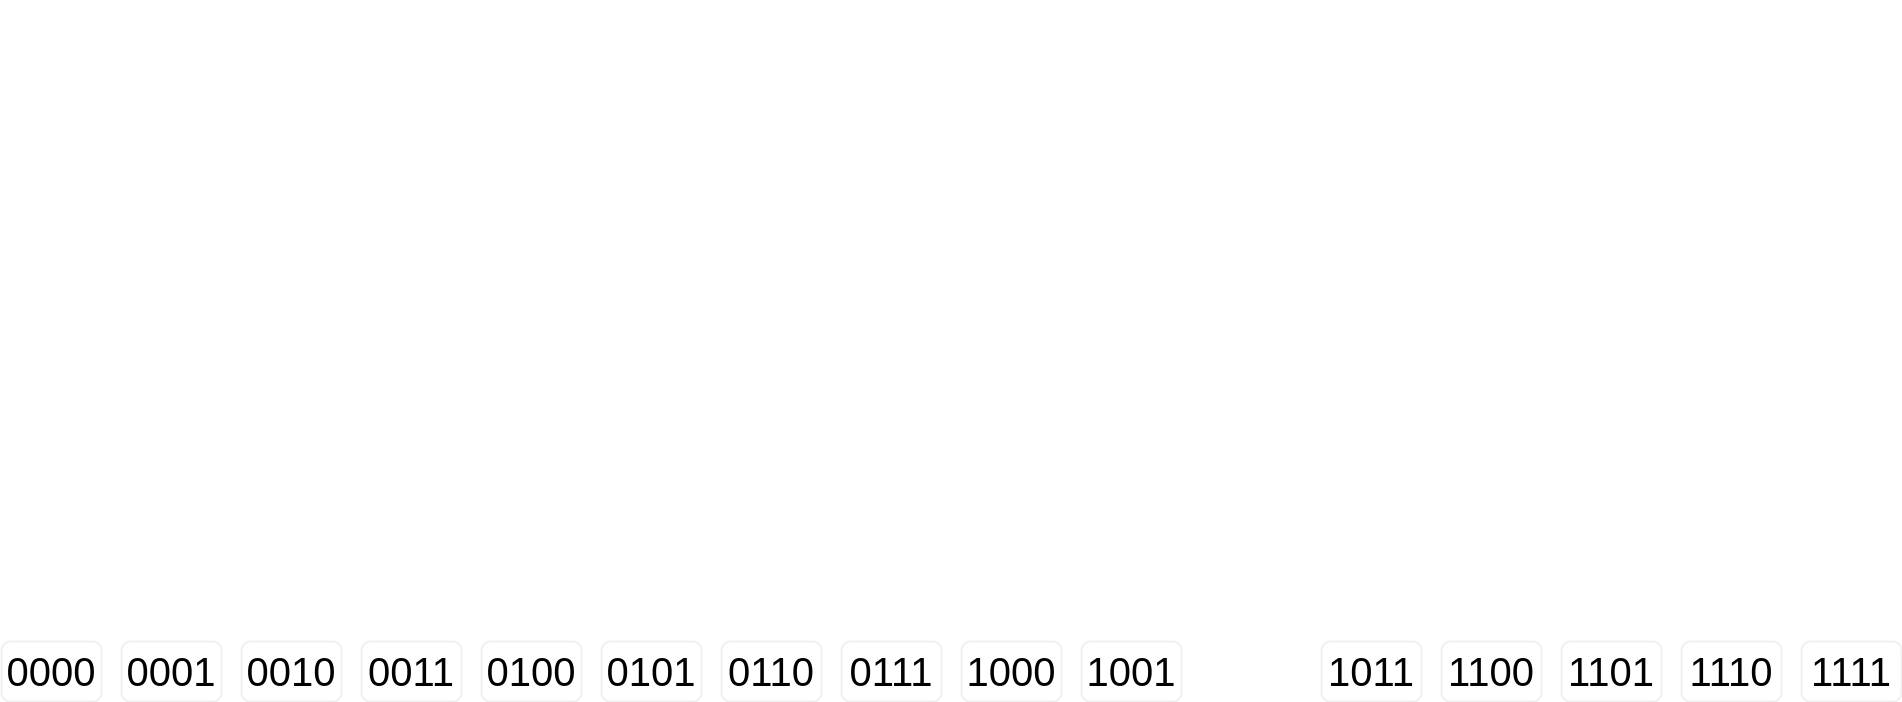
\includegraphics[width=\linewidth,keepaspectratio]{resources/dht-insert0.png}
\end{center}
\end{minipage}
\end{frame}

\begin{frame}
\frametitle{Joining the DHT}
\begin{minipage}[b]{\linewidth}
\begin{center}
        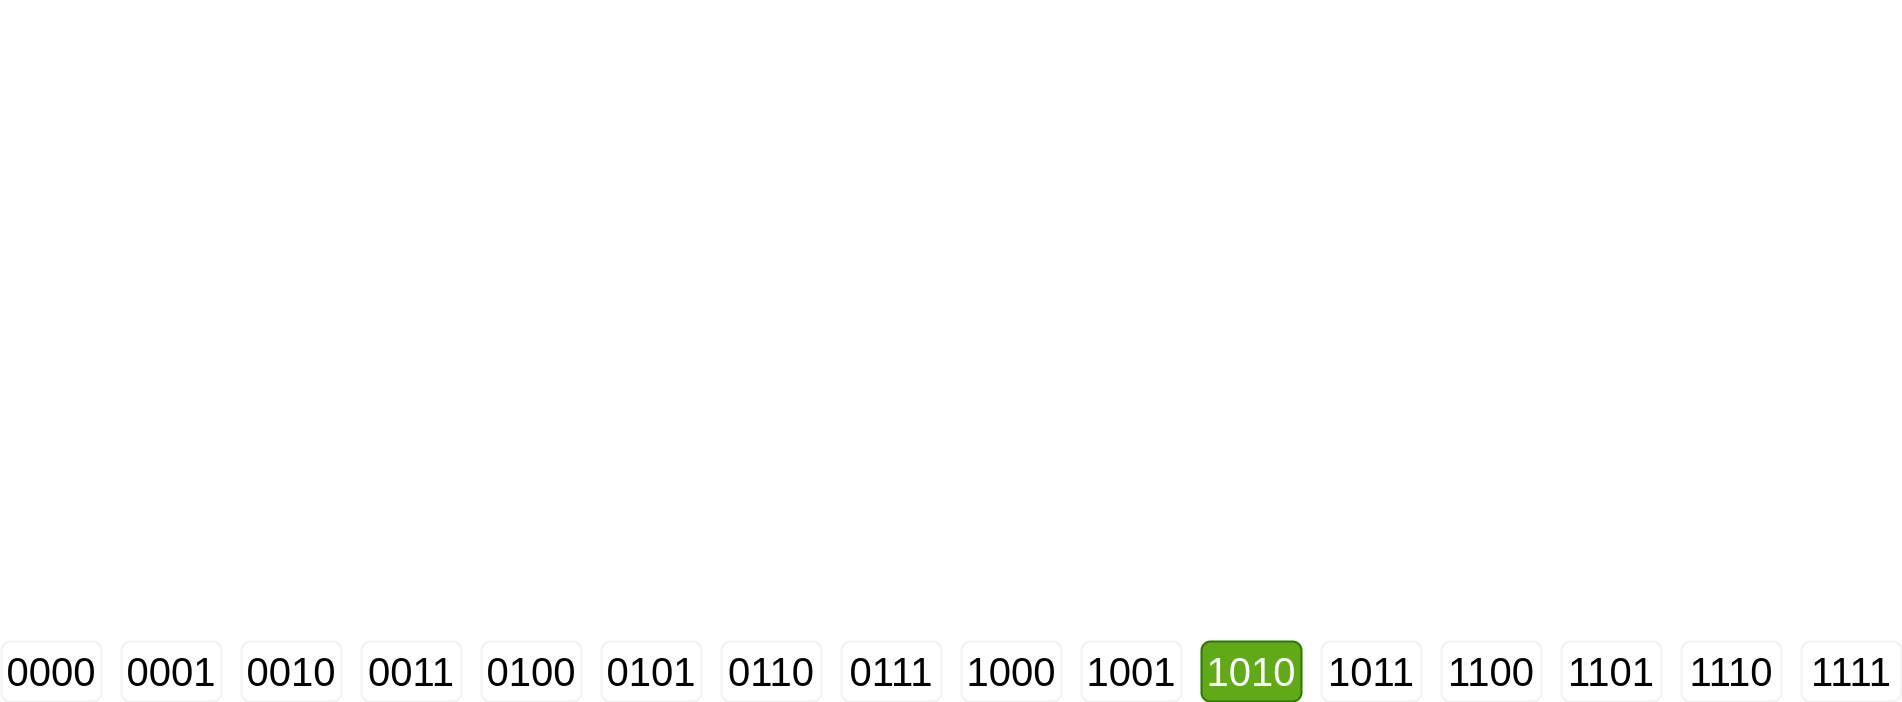
\includegraphics[width=\linewidth,keepaspectratio]{resources/dht-insert1.png}
\end{center}
\end{minipage}
\end{frame}


\begin{frame}
\frametitle{Joining the DHT}
\begin{minipage}[b]{\linewidth}
\begin{center}
        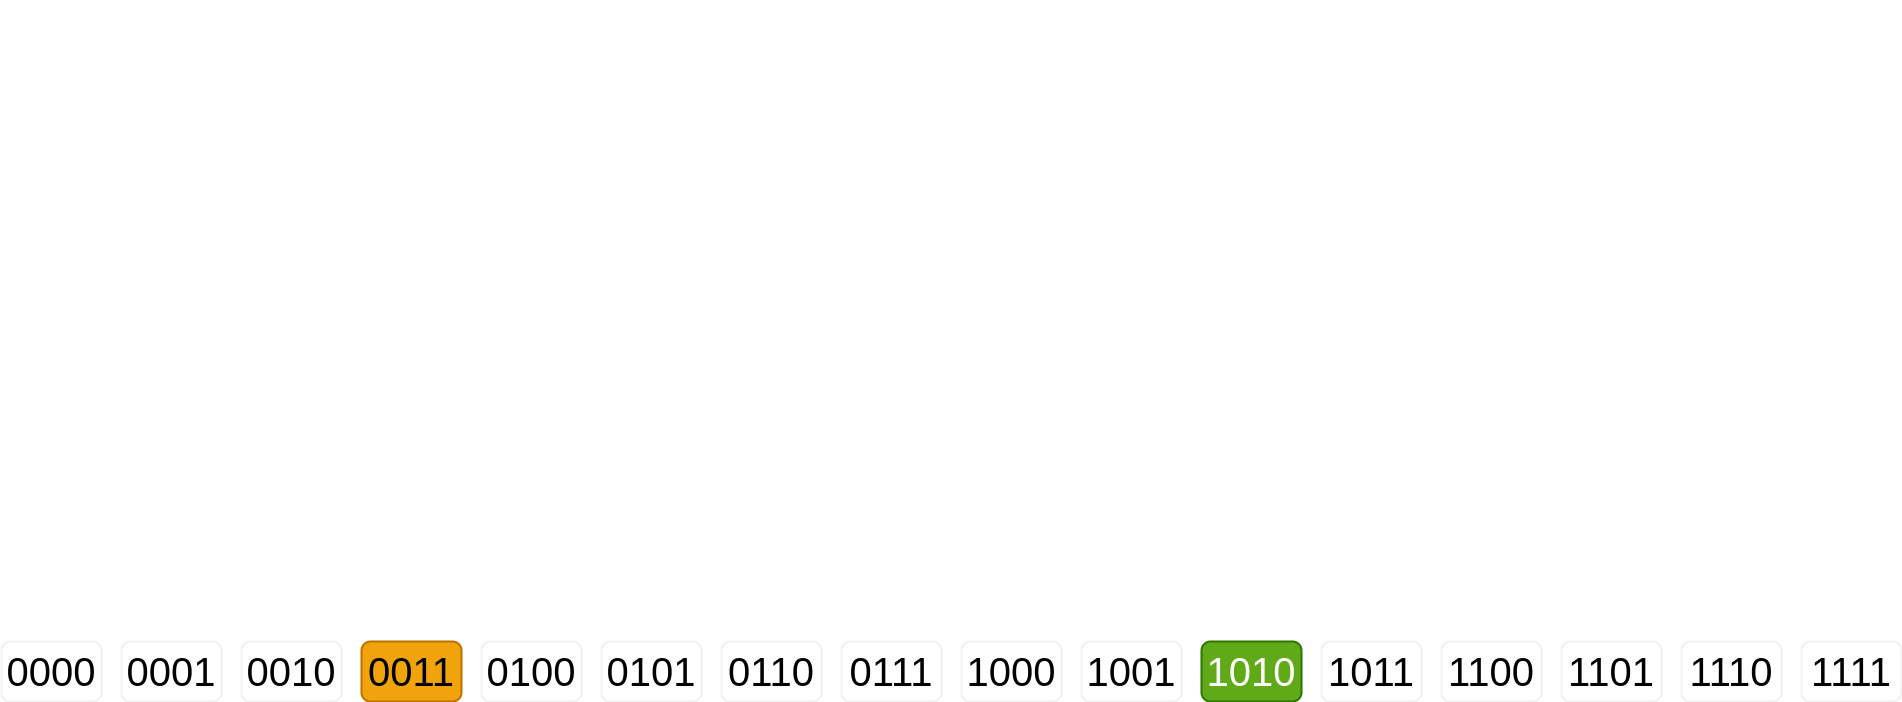
\includegraphics[width=\linewidth,keepaspectratio]{resources/dht-insert.png}
\end{center}
\end{minipage}
\end{frame}

\begin{frame}
\frametitle{Joining the DHT: self lookup}
\begin{minipage}[b]{\linewidth}
\begin{center}
        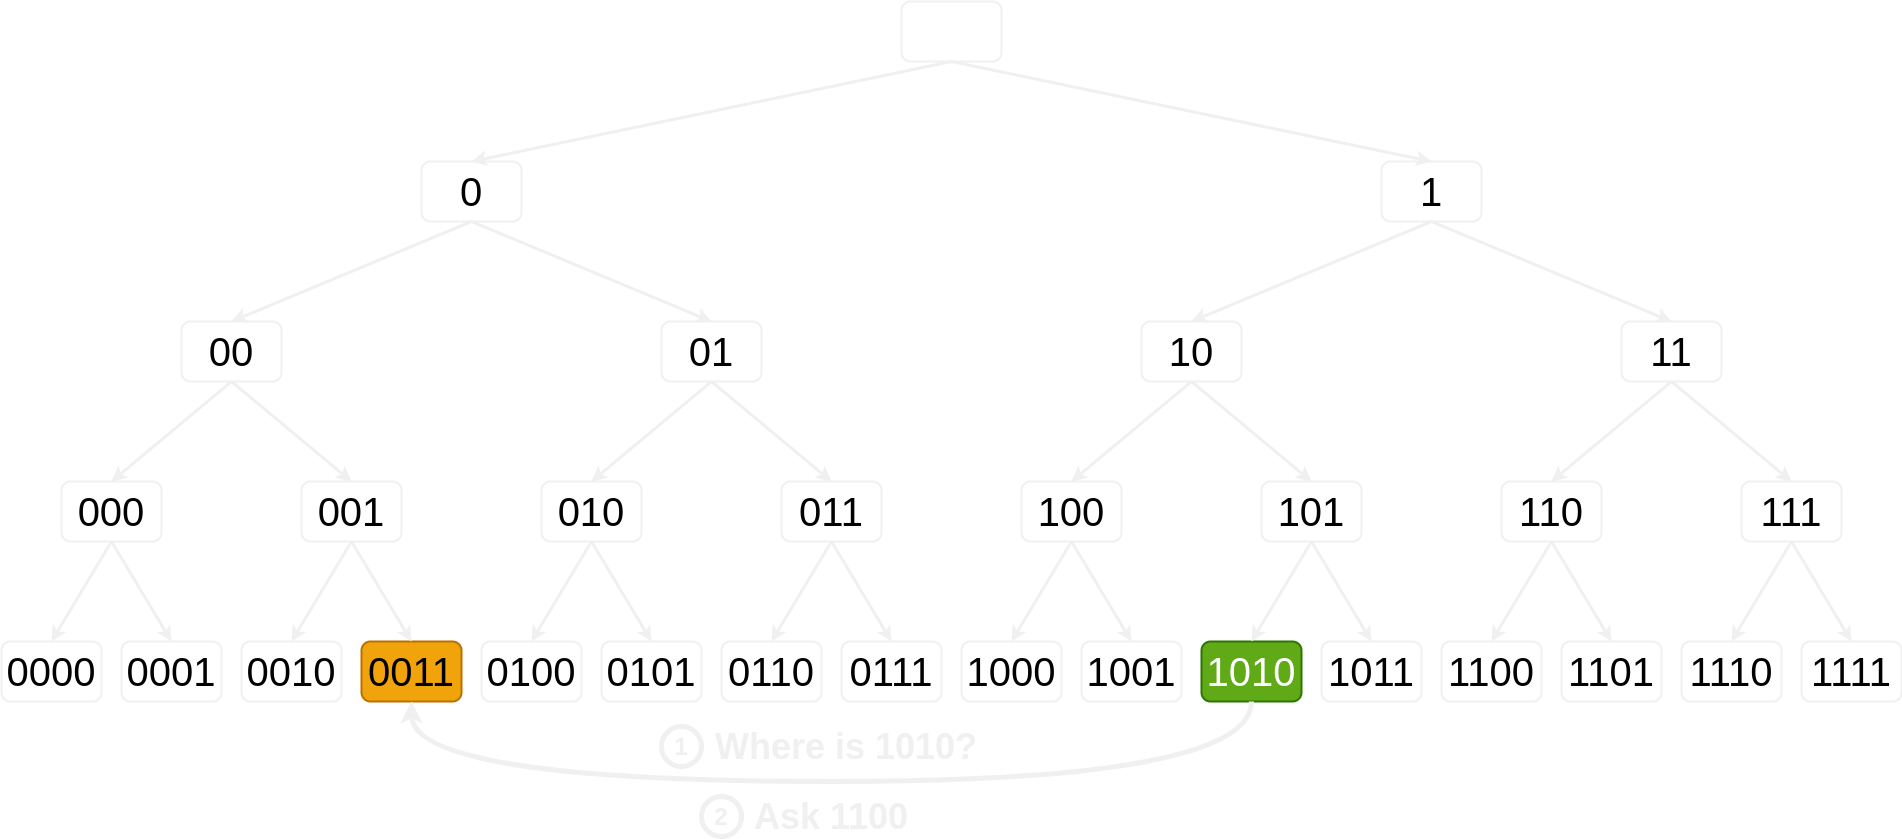
\includegraphics[width=\linewidth,keepaspectratio]{resources//dht-self-lookup.png}
\end{center}
\end{minipage}
\end{frame}

\begin{frame}
\frametitle{Joining the DHT: self lookup}
\begin{minipage}[b]{\linewidth}
\begin{center}
        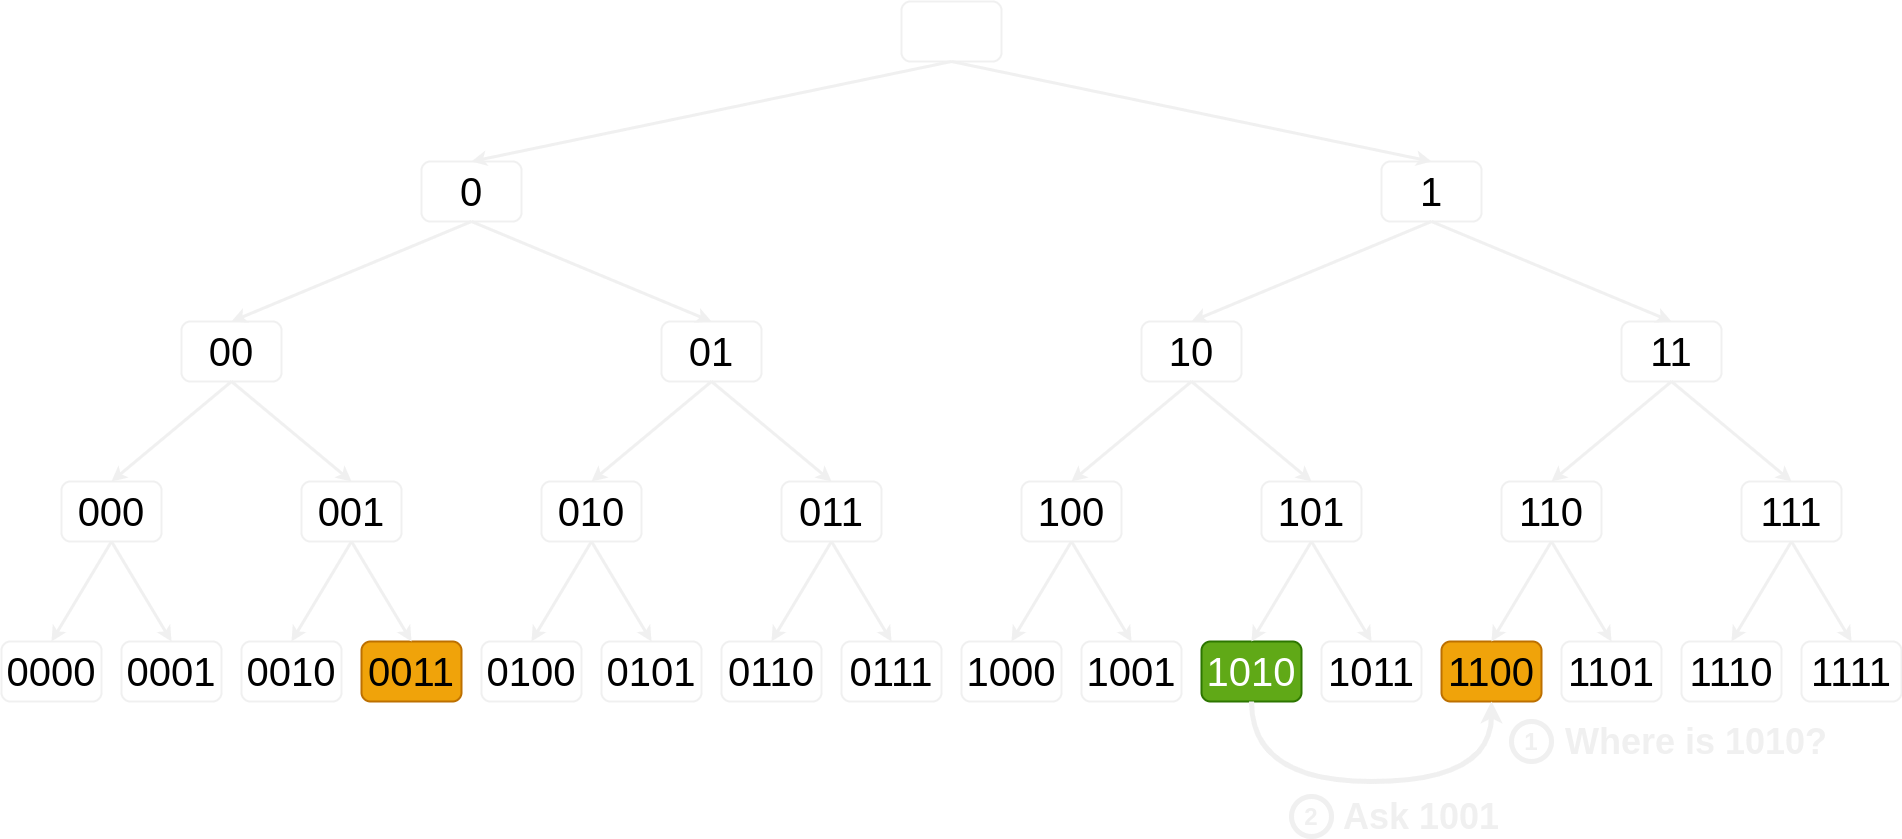
\includegraphics[width=\linewidth,keepaspectratio]{resources//dht-self-lookup2.png}
\end{center}
\end{minipage}
\end{frame}

\begin{frame}
\frametitle{Joining the DHT: self lookup}
\begin{minipage}[b]{\linewidth}
\begin{center}
        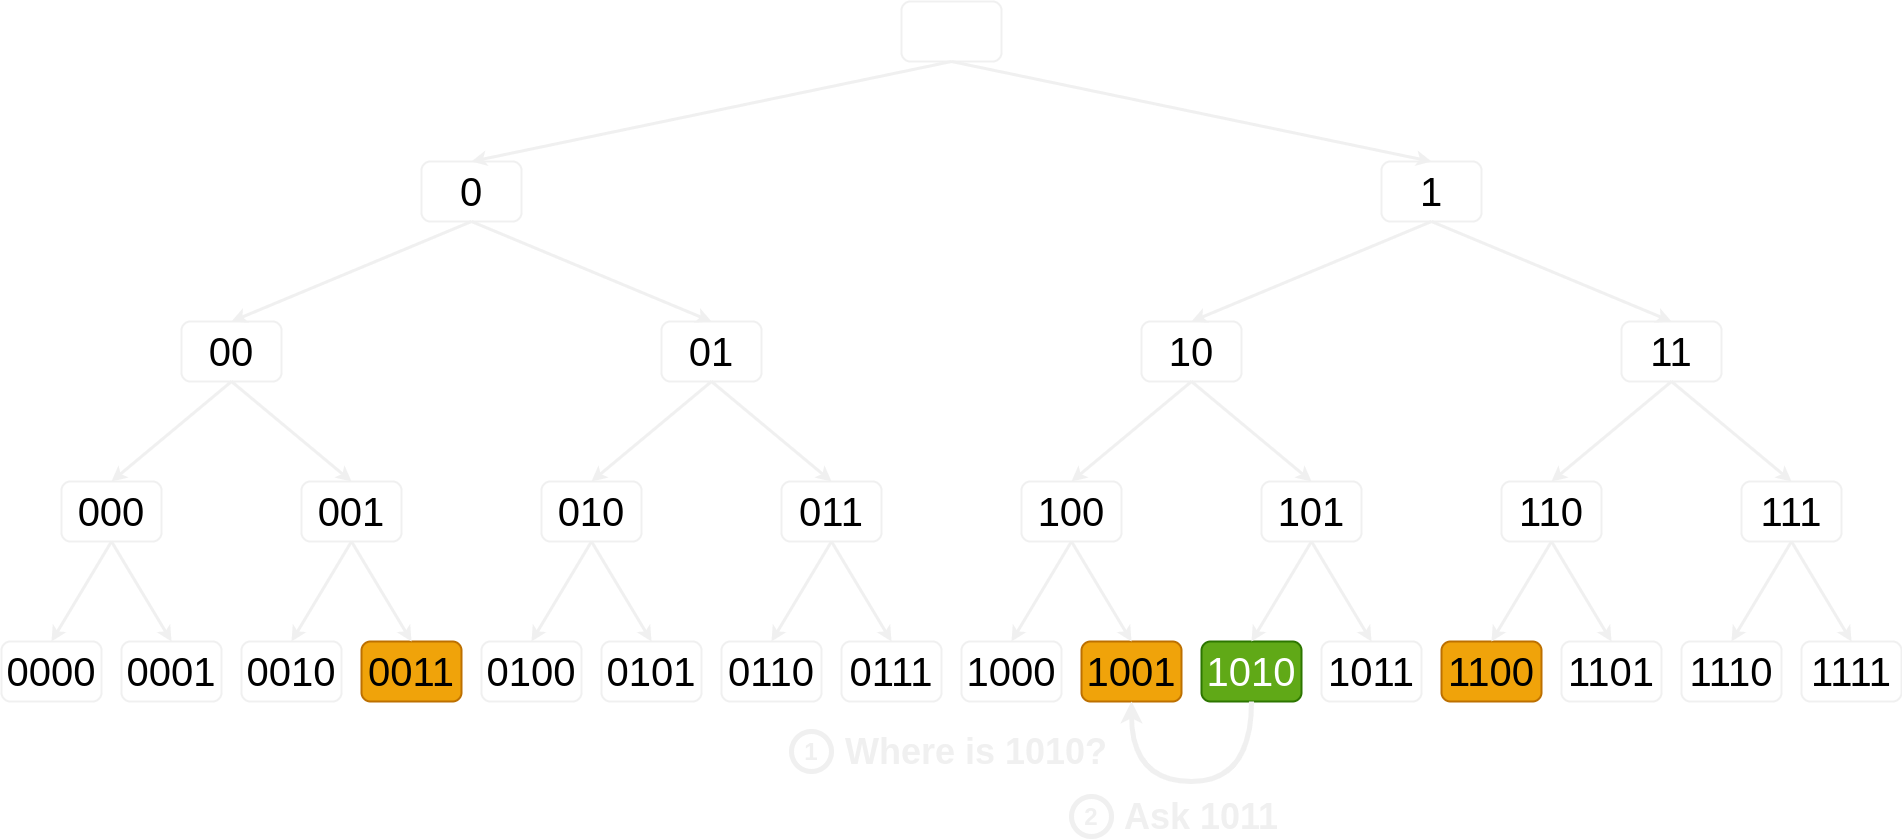
\includegraphics[width=\linewidth,keepaspectratio]{resources//dht-self-lookup3.png}
\end{center}
\end{minipage}
\end{frame}

\begin{frame}
\frametitle{Joining the DHT: self lookup}
\begin{minipage}[b]{\linewidth}
\begin{center}
        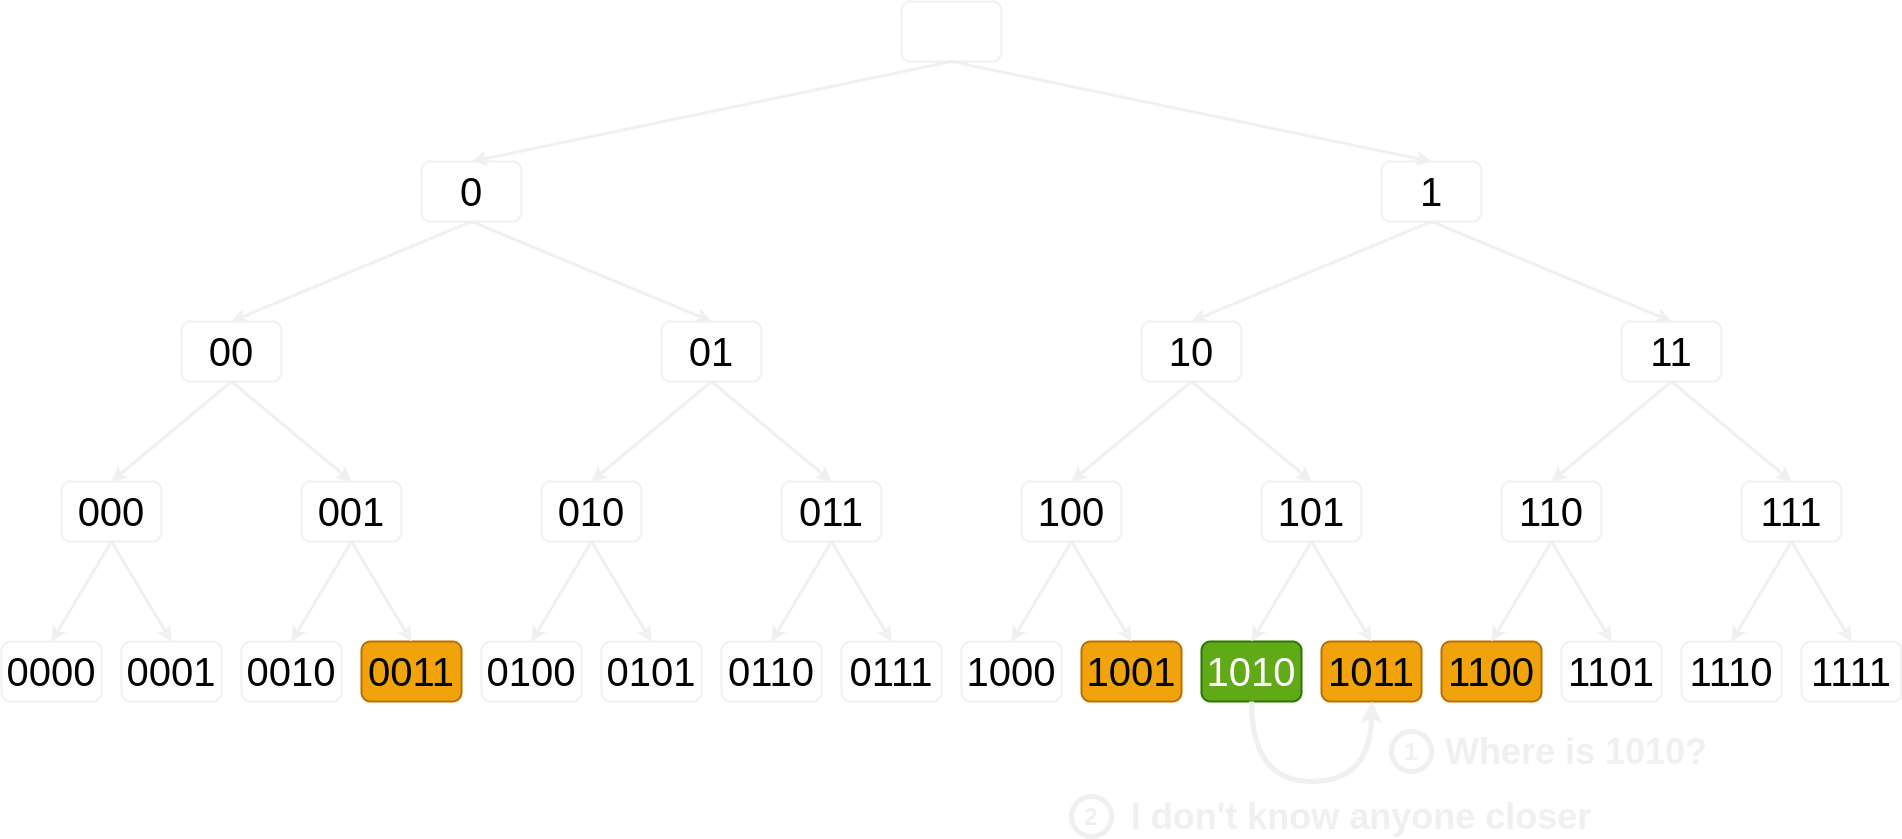
\includegraphics[width=\linewidth,keepaspectratio]{resources//dht-self-lookup4.png}
\end{center}
\end{minipage}
\end{frame}


\begin{frame}
\frametitle{Kademlia details}
\begin{itemize}
	\itemc Each node periodically looks up for its own \texttt{PeerID}
	\itemc Multiple requests happen concurrently for the same key
	\itemc Upon request a peer returns the 20 closest peers it knows to the requested key
	\itemc When a Provider Records is published to the DHT it is stored on the 20 closest peers to its key
	\itemc Buckets are capped at 20 peers
	\bigskip
	\itemc \textbf{These constants don't need to be the same value!}
	\end{itemize}
\end{frame}

\begin{frame}
\frametitle{Kademlia keyspace}
\begin{tikzpicture}[
	thick,
	scale=0.8,
  	every node/.style={scale=0.8},
    level 1/.style = {sibling distance=8.8cm},
    level 2/.style = {sibling distance=4.4cm},
    level 3/.style = {sibling distance=2.2cm},
    level 4/.style = {sibling distance=1.1cm},
    level distance = 1.5cm
]
 	\node[trienode] {root}
	child {
		node[trienode] (n0) {0}
		child {
			node[trienode] {00}
			child {
				node[trienode] {000}
				child {
					node[trienode] {0000}
				}
				child {
					node[trienode] {0001}
				}
			}
			child {
				node[trienode] {001}
				child {
					node[trienode] {0010}
				}
				child {
					node[trienode] {0011}
				}
			}
		}
		child {
			node[trienode] {01}
			child {
				node[trienode] {010}
				child {
					node[trienode] {0100}
				}
				child {
					node[trienode] {0101}
				}
			}
			child {
				node[trienode] {011}
				child {
					node[trienode] {0110}
				}
				child {
					node[trienode] {0111}
				}
			}
		}
	}
	child {
		node[trienode] {1}
		child {
			node[trienode] {10}
			child {
				node[trienode] (n100) {100}
				child {
					node[trienode] {1000}
				}
				child {
					node[trienode] {1001}
				}
			}
			child {
				node[trienode] {101}
				child {
					node[trienode] (n1010) {1010}
				}
				child {
					node[trienode] (n1011) {1011}
				}
			}
		}
		child {
			node[trienode] (n11) {11}
			child {
				node[trienode] {110}
				child {
					node[trienode] {1100}
				}
				child {
					node[trienode] {1101}
				}
			}
			child {
				node[trienode] {111}
				child {
					node[trienode] {1110}
				}
				child {
					node[trienode] {1111}
				}
			}
		}
	};
\end{tikzpicture}
\end{frame}

\begin{frame}
\frametitle{Kademlia keyspace}
\begin{tikzpicture}[
	thick,
	scale=0.8,
  	every node/.style={scale=0.8},
    level 1/.style = {sibling distance=8.8cm},
    level 2/.style = {sibling distance=4.4cm},
    level 3/.style = {sibling distance=2.2cm},
    level 4/.style = {sibling distance=1.1cm},
    level distance = 1.5cm
]
 	\node[trienode] {root}
	child {
		node[trienode] (n0) {0}
		child {
			node[trienode] {00}
			child {
				node[trienode] {000}
				child {
					node[trienode] {0000}
				}
				child {
					node[trienode] {0001}
				}
			}
			child {
				node[trienode] {001}
				child {
					node[trienode] {0010}
				}
				child {
					node[trienode] {0011}
				}
			}
		}
		child {
			node[trienode] {01}
			child {
				node[trienode] {010}
				child {
					node[trienode] {0100}
				}
				child {
					node[trienode] {0101}
				}
			}
			child {
				node[trienode] {011}
				child {
					node[trienode] {0110}
				}
				child {
					node[trienode] {0111}
				}
			}
		}
	}
	child {
		node[trienode] {1}
		child {
			node[trienode] {10}
			child {
				node[trienode] (n100) {100}
				child {
					node[trienode] {1000}
				}
				child {
					node[trienode] {1001}
				}
			}
			child {
				node[trienode] {101}
				child {
					node[trienode] (n1010) {\textbf{1010}}
				}
				child {
					node[trienode] (n1011) {1011}
				}
			}
		}
		child {
			node[trienode] (n11) {11}
			child {
				node[trienode] {110}
				child {
					node[trienode] {1100}
				}
				child {
					node[trienode] {1101}
				}
			}
			child {
				node[trienode] {111}
				child {
					node[trienode] {1110}
				}
				child {
					node[trienode] {1111}
				}
			}
		}
	};
	\node[below=of n1010] (ref) {Reference node};
	\draw[->,thick] (ref) -- (n1010);
\end{tikzpicture}
\end{frame}

\begin{frame}
\frametitle{Kademlia keyspace}
\begin{tikzpicture}[
	thick,
	scale=0.8,
  	every node/.style={scale=0.8},
    level 1/.style = {sibling distance=8.8cm},
    level 2/.style = {sibling distance=4.4cm},
    level 3/.style = {sibling distance=2.2cm},
    level 4/.style = {sibling distance=1.1cm},
    level distance = 1.5cm
]
 	\node[trienode] {root}
	child {
		node[trienode] (n0) {0}
		child {
			node[trienode] {00}
			child {
				node[trienode] {000}
				child {
					node[trienode] {0000}
				}
				child {
					node[trienode] {0001}
				}
			}
			child {
				node[trienode] {001}
				child {
					node[trienode] {0010}
				}
				child {
					node[trienode] {0011}
				}
			}
		}
		child {
			node[trienode] {01}
			child {
				node[trienode] {010}
				child {
					node[trienode] {0100}
				}
				child {
					node[trienode] {0101}
				}
			}
			child {
				node[trienode] {011}
				child {
					node[trienode] {0110}
				}
				child {
					node[trienode] {0111}
				}
			}
		}
	}
	child {
		node[trienode] {1}
		child {
			node[trienode] {10}
			child {
				node[trienode] (n100) {100}
				child {
					node[trienode] {1000}
				}
				child {
					node[trienode] {1001}
				}
			}
			child {
				node[trienode] {{101}}
				child {
					node[trienode] (n1010) {\textbf{1010}}
				}
				child {
					node[trienode] (n1011) {{101}1}
				}
			}
		}
		child {
			node[trienode] (n11) {11}
			child {
				node[trienode] {110}
				child {
					node[trienode] {1100}
				}
				child {
					node[trienode] {1101}
				}
			}
			child {
				node[trienode] {111}
				child {
					node[trienode] {1110}
				}
				child {
					node[trienode] {1111}
				}
			}
		}
	};
	\node[bucket, above=of n0, yshift=-6.5cm, minimum width=8.8cm, minimum height=5.4cm, label=below:bucket0] {};
	\node[below=of n1010] (ref) {Reference node};
	\draw[->,thick] (ref) -- (n1010);
\end{tikzpicture}
\end{frame}


\begin{frame}
\frametitle{Kademlia keyspace}
\begin{tikzpicture}[
	thick,
	scale=0.8,
  	every node/.style={scale=0.8},
    level 1/.style = {sibling distance=8.8cm},
    level 2/.style = {sibling distance=4.4cm},
    level 3/.style = {sibling distance=2.2cm},
    level 4/.style = {sibling distance=1.1cm},
    level distance = 1.5cm
]
 	\node[trienode] {root}
	child {
		node[trienode] (n0) {0}
		child {
			node[trienode] {00}
			child {
				node[trienode] {000}
				child {
					node[trienode] {0000}
				}
				child {
					node[trienode] {0001}
				}
			}
			child {
				node[trienode] {001}
				child {
					node[trienode] {0010}
				}
				child {
					node[trienode] {0011}
				}
			}
		}
		child {
			node[trienode] {01}
			child {
				node[trienode] {010}
				child {
					node[trienode] {0100}
				}
				child {
					node[trienode] {0101}
				}
			}
			child {
				node[trienode] {011}
				child {
					node[trienode] {0110}
				}
				child {
					node[trienode] {0111}
				}
			}
		}
	}
	child {
		node[trienode] {1}
		child {
			node[trienode] {{10}}
			child {
				node[trienode] (n100) {{10}0}
				child {
					node[trienode] {{10}00}
				}
				child {
					node[trienode] {{10}01}
				}
			}
			child {
				node[trienode] {{101}}
				child {
					node[trienode] (n1010) {\textbf{1010}}
				}
				child {
					node[trienode] (n1011) {{101}1}
				}
			}
		}
		child {
			node[trienode] (n11) {\textbf{1}1}
			child {
				node[trienode] {\textbf{1}10}
				child {
					node[trienode] {\textbf{1}100}
				}
				child {
					node[trienode] {\textbf{1}101}
				}
			}
			child {
				node[trienode] {\textbf{1}11}
				child {
					node[trienode] {\textbf{1}110}
				}
				child {
					node[trienode] {\textbf{1}111}
				}
			}
		}
	};
	\node[bucket, above=of n0, yshift=-6.5cm, minimum width=8.8cm, minimum height=5.4cm, label=below:bucket0] {};
	\node[bucket, above=of n11, yshift=-5cm, minimum width=4.4cm, minimum height=4cm, label=below:bucket1] {};
	\node[below=of n1010] (ref) {Reference node};
	\draw[->,thick] (ref) -- (n1010);
\end{tikzpicture}
\end{frame}

\begin{frame}
\frametitle{Kademlia keyspace}
\begin{tikzpicture}[
	thick,
	scale=0.8,
  	every node/.style={scale=0.8},
    level 1/.style = {sibling distance=8.8cm},
    level 2/.style = {sibling distance=4.4cm},
    level 3/.style = {sibling distance=2.2cm},
    level 4/.style = {sibling distance=1.1cm},
    level distance = 1.5cm
]
 	\node[trienode] {root}
	child {
		node[trienode] (n0) {0}
		child {
			node[trienode] {00}
			child {
				node[trienode] {000}
				child {
					node[trienode] {0000}
				}
				child {
					node[trienode] {0001}
				}
			}
			child {
				node[trienode] {001}
				child {
					node[trienode] {0010}
				}
				child {
					node[trienode] {0011}
				}
			}
		}
		child {
			node[trienode] {01}
			child {
				node[trienode] {010}
				child {
					node[trienode] {0100}
				}
				child {
					node[trienode] {0101}
				}
			}
			child {
				node[trienode] {011}
				child {
					node[trienode] {0110}
				}
				child {
					node[trienode] {0111}
				}
			}
		}
	}
	child {
		node[trienode] {{1}}
		child {
			node[trienode] {{10}}
			child {
				node[trienode] (n100) {\textbf{10}0}
				child {
					node[trienode] {\textbf{10}00}
				}
				child {
					node[trienode] {\textbf{10}01}
				}
			}
			child {
				node[trienode] {{101}}
				child {
					node[trienode] (n1010) {\textbf{1010}}
				}
				child {
					node[trienode] (n1011) {{101}1}
				}
			}
		}
		child {
			node[trienode] (n11) {\textbf{1}1}
			child {
				node[trienode] {\textbf{1}10}
				child {
					node[trienode] {\textbf{1}100}
				}
				child {
					node[trienode] {\textbf{1}101}
				}
			}
			child {
				node[trienode] {\textbf{1}11}
				child {
					node[trienode] {\textbf{1}110}
				}
				child {
					node[trienode] {\textbf{1}111}
				}
			}
		}
	};
	\node[bucket, above=of n0, yshift=-6.5cm, minimum width=8.8cm, minimum height=5.4cm, label=below:bucket0] {};
	\node[bucket, above=of n11, yshift=-5cm, minimum width=4.4cm, minimum height=4cm, label=below:bucket1] {};
	\node[bucket, above=of n100, yshift=-3.5cm, minimum width=2.2cm, minimum height=2.5cm, label=below:bucket2] {};
	\node[below=of n1010] (ref) {Reference node};
	\draw[->,thick] (ref) -- (n1010);
\end{tikzpicture}
\end{frame}

\begin{frame}
\frametitle{Kademlia keyspace}
\begin{tikzpicture}[
	thick,
	scale=0.8,
  	every node/.style={scale=0.8},
    level 1/.style = {sibling distance=8.8cm},
    level 2/.style = {sibling distance=4.4cm},
    level 3/.style = {sibling distance=2.2cm},
    level 4/.style = {sibling distance=1.1cm},
    level distance = 1.5cm
]
 	\node[trienode] {root}
	child {
		node[trienode] (n0) {0}
		child {
			node[trienode] {00}
			child {
				node[trienode] {000}
				child {
					node[trienode] {0000}
				}
				child {
					node[trienode] {0001}
				}
			}
			child {
				node[trienode] {001}
				child {
					node[trienode] {0010}
				}
				child {
					node[trienode] {0011}
				}
			}
		}
		child {
			node[trienode] {01}
			child {
				node[trienode] {010}
				child {
					node[trienode] {0100}
				}
				child {
					node[trienode] {0101}
				}
			}
			child {
				node[trienode] {011}
				child {
					node[trienode] {0110}
				}
				child {
					node[trienode] {0111}
				}
			}
		}
	}
	child {
		node[trienode] {\textbf{1}}
		child {
			node[trienode] {\textbf{10}}
			child {
				node[trienode] (n100) {\textbf{10}0}
				child {
					node[trienode] {\textbf{10}00}
				}
				child {
					node[trienode] {\textbf{10}01}
				}
			}
			child {
				node[trienode] {\textbf{101}}
				child {
					node[trienode] (n1010) {\textbf{1010}}
				}
				child {
					node[trienode] (n1011) {\textbf{101}1}
				}
			}
		}
		child {
			node[trienode] (n11) {\textbf{1}1}
			child {
				node[trienode] {\textbf{1}10}
				child {
					node[trienode] {\textbf{1}100}
				}
				child {
					node[trienode] {\textbf{1}101}
				}
			}
			child {
				node[trienode] {\textbf{1}11}
				child {
					node[trienode] {\textbf{1}110}
				}
				child {
					node[trienode] {\textbf{1}111}
				}
			}
		}
	};
	\node[bucket, above=of n0, yshift=-6.5cm, minimum width=8.8cm, minimum height=5.4cm, label=below:bucket0] {};
	\node[bucket, above=of n11, yshift=-5cm, minimum width=4.4cm, minimum height=4cm, label=below:bucket1] {};
	\node[bucket, above=of n100, yshift=-3.5cm, minimum width=2.2cm, minimum height=2.5cm, label=below:bucket2] {};
	\node[bucket, above=of n1011, yshift=-2cm, minimum width=1.1cm, minimum height=1cm, label=below:bucket3] {};
	\node[below=of n1010] (ref) {Reference node};
	\draw[->,thick] (ref) -- (n1010);
\end{tikzpicture}
\end{frame}


\begin{frame}
\frametitle{Example: Routing Table of peer \texttt{01101000}}
\begin{columns}[onlytextwidth,t]
\begin{column}{0.19\textwidth}
	\textbf{Bucket 0}
   	\begin{enumerate}
   		\item 11010111
   		\item 10001011
   		\item 10101110
   		\item 11110101
   		\item 10000010
   		\item 11010100
   		\item 11000100
   		\item ...
   	\end{enumerate}
\end{column}
\begin{column}{0.19\textwidth}
	\textbf{Bucket 1}
   \begin{enumerate}
   		\item \textbf{0}0110101
   		\item \textbf{0}0001000
   		\item \textbf{0}0111011
   		\item \textbf{0}0101101
   		\item \textbf{0}0110100
   \end{enumerate}
\end{column}
\begin{column}{0.19\textwidth}
	\textbf{Bucket 2}
   \begin{enumerate}
   		\item \textbf{01}011101
   		\item \textbf{01}001111
   		\item \textbf{01}010110
   \end{enumerate}
\end{column}
\begin{column}{0.19\textwidth}
	\textbf{Bucket 3}
   \begin{enumerate}
   		\item \textbf{011}11011
   		\item \textbf{011}10001
   \end{enumerate}
\end{column}
\begin{column}{0.19\textwidth}
	\textbf{Bucket 4}
   	\begin{enumerate}
   		\item \textbf{0110}0011
   \end{enumerate}
\end{column}
\end{columns}
\end{frame}

\begin{frame}
\frametitle{\texttt{k-bucket} replacement policy}
\begin{itemize}
    \itemc \texttt{Kademlia}: only when a bucket is full and there is a new candidate, least-recently seen and unreachable node gets evicted, but live nodes are never evicted
	\bigskip    
    \itemc \texttt{kubo} implementation: periodically ping the nodes in the routing table, and evict the unresponsive ones
\end{itemize}
\end{frame}

\begin{frame}
\frametitle{Measurements data}
\begin{itemize}
    \itemc The Nebula Crawler crawls the IPFS network and provides all peers in the network along with their routing table for a point in time
    \itemc Data taken from 28 crawls over 1 week (4 crawls per day) starting on \texttt{2022-04-19}
\end{itemize}
\end{frame}

\begin{frame}
\frametitle{Methodology}
\begin{itemize}
	\itemc The Nebula Crawler provides a global snapshot of the network
	\itemc We can reconstruct the \texttt{k-buckets} of all peers by computing the XOR distance between a \texttt{PeerID} and the \texttt{PeerID}s of all peers in its routing table
	\itemc From the global snapshot we can find the closest peers to every other peer and verify if any peer is missing from a \texttt{k-bucket}
    %\itemc Caveat: XOR distance is non-linear! Computationnaly expensive to find the closest peers to a specific \texttt{peer\_id}. A python Binary Trie implementation was built for this purpose
\end{itemize}
\end{frame}


\begin{frame}
\frametitle{Unreachable peers in the Routing Table}

\begin{columns}[onlytextwidth]
\begin{column}{0.38\textwidth}
Unreachable peers may still be referenced in other peers routing tables (stale entries)
\bigskip
   \begin{itemize}
   		\itemc Average for buckets \texttt{0} to \texttt{8}: \texttt{3.8\%} $\sim$ \texttt{0.75} peers
   		\itemc Average for buckets \texttt{9} to \texttt{21}: \texttt{15\%}
   \end{itemize}
\end{column}
\begin{column}{0.58\textwidth}
    \begin{center}
		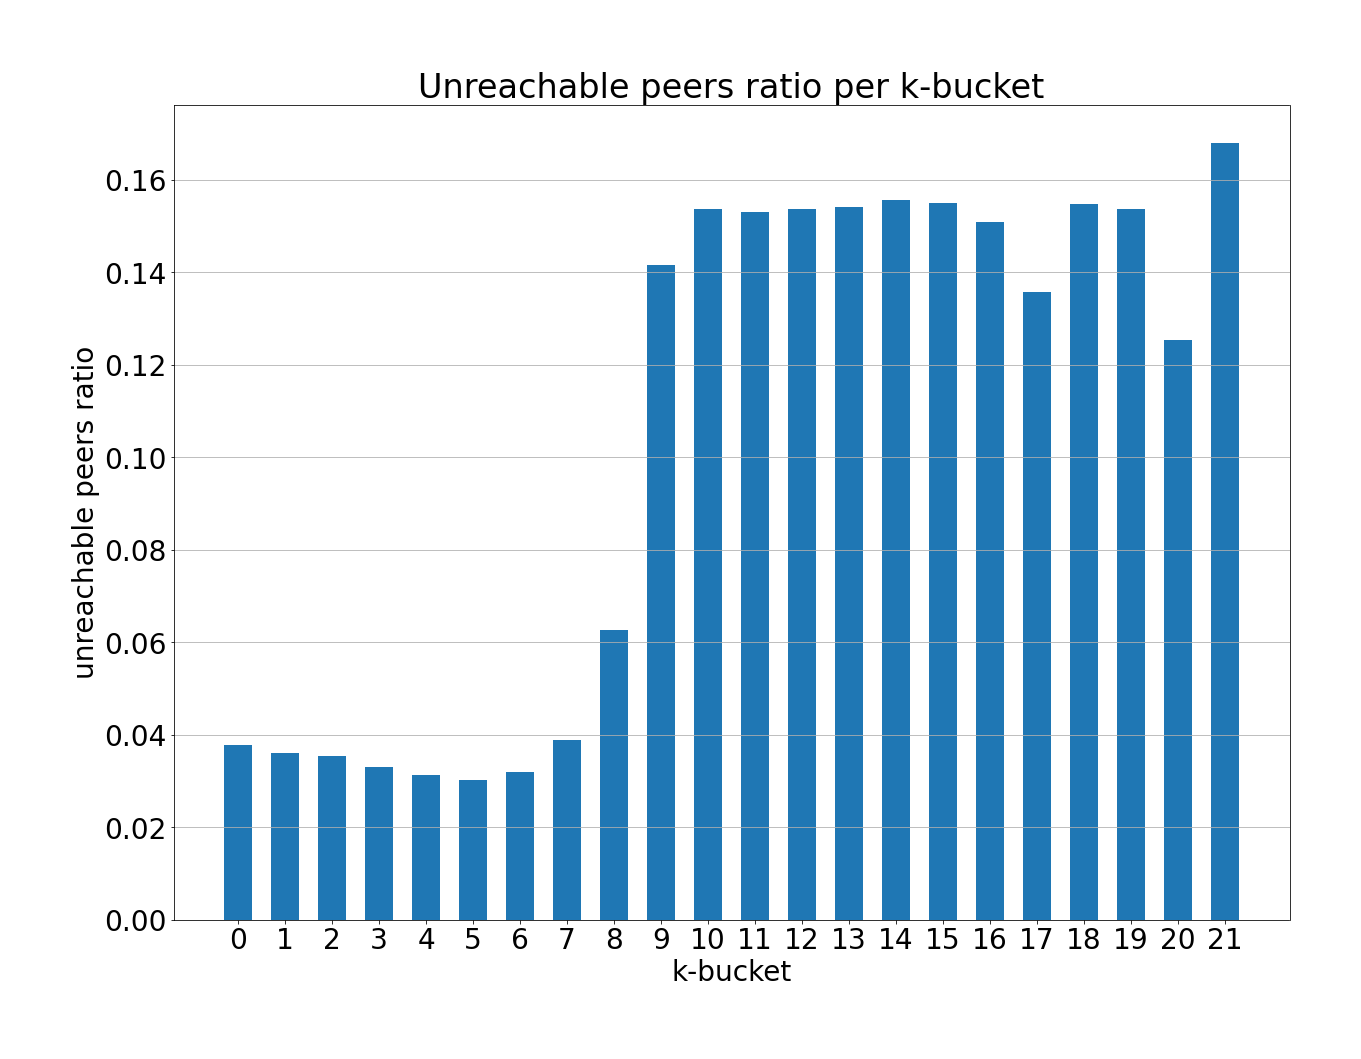
\includegraphics[width=\textwidth]{plots/unreachable-peers.png}
    \end{center}
\end{column}
\end{columns}
\end{frame}

\begin{frame}
\frametitle{Peers distribution in the k-buckets}

\begin{columns}[onlytextwidth]
\begin{column}{0.38\textwidth}
   	\begin{itemize}
   		\itemc Peers distribution in bucket follows an exponential growth, capped at 20
   		\itemc Buckets \texttt{0-8} are missing on average \texttt{0.12} peers per bucket
   		\itemc Buckets \texttt{9-14} are missing on average \texttt{0.53} peers per bucket
   	\end{itemize}
\end{column}
\begin{column}{0.58\textwidth}
    \begin{center}
		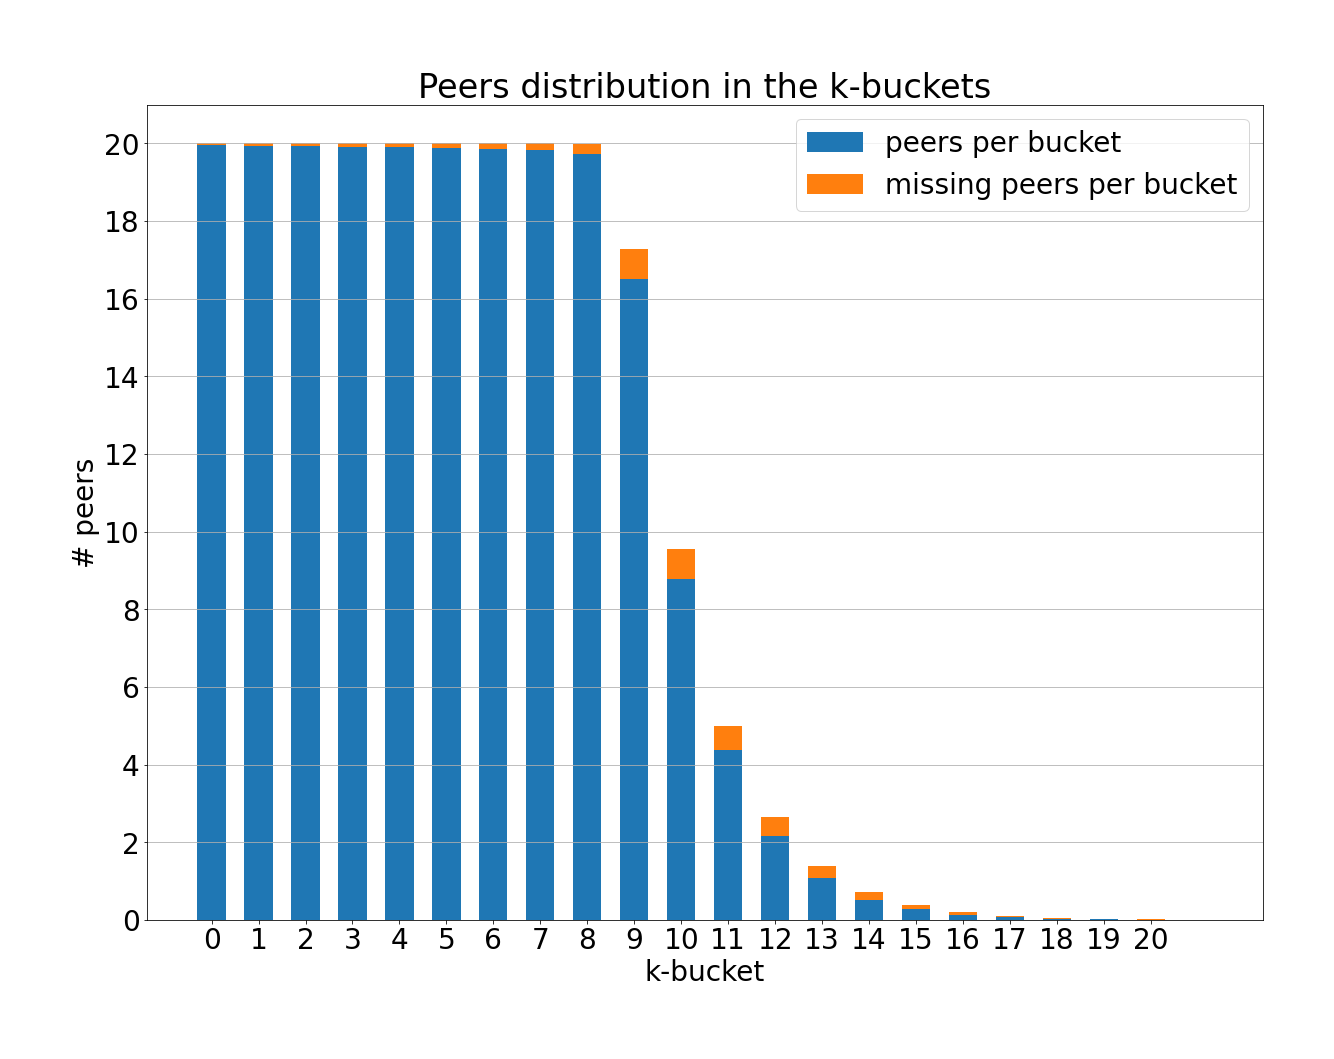
\includegraphics[width=\textwidth]{plots/peers-distribution-including-missing.png}
    \end{center}
\end{column}
\end{columns}
\end{frame}


\begin{frame}
\frametitle{20 closest peers awareness}

\begin{columns}[onlytextwidth]
\begin{column}{0.38\textwidth}
\begin{enumerate}
   	\itemc Probability Density Function (PDF)
   	\itemc Cumulative Distribution Function (CDF)
\end{enumerate}
\bigskip
\begin{itemize}
   	\itemc \texttt{61.1\%} of the peers know all their 20 closest peers
   	\itemc \texttt{95.2\%} of the peers know at least 18 of their 20 closest peers
\end{itemize}
\end{column}
\begin{column}{0.58\textwidth}
    \begin{center}
		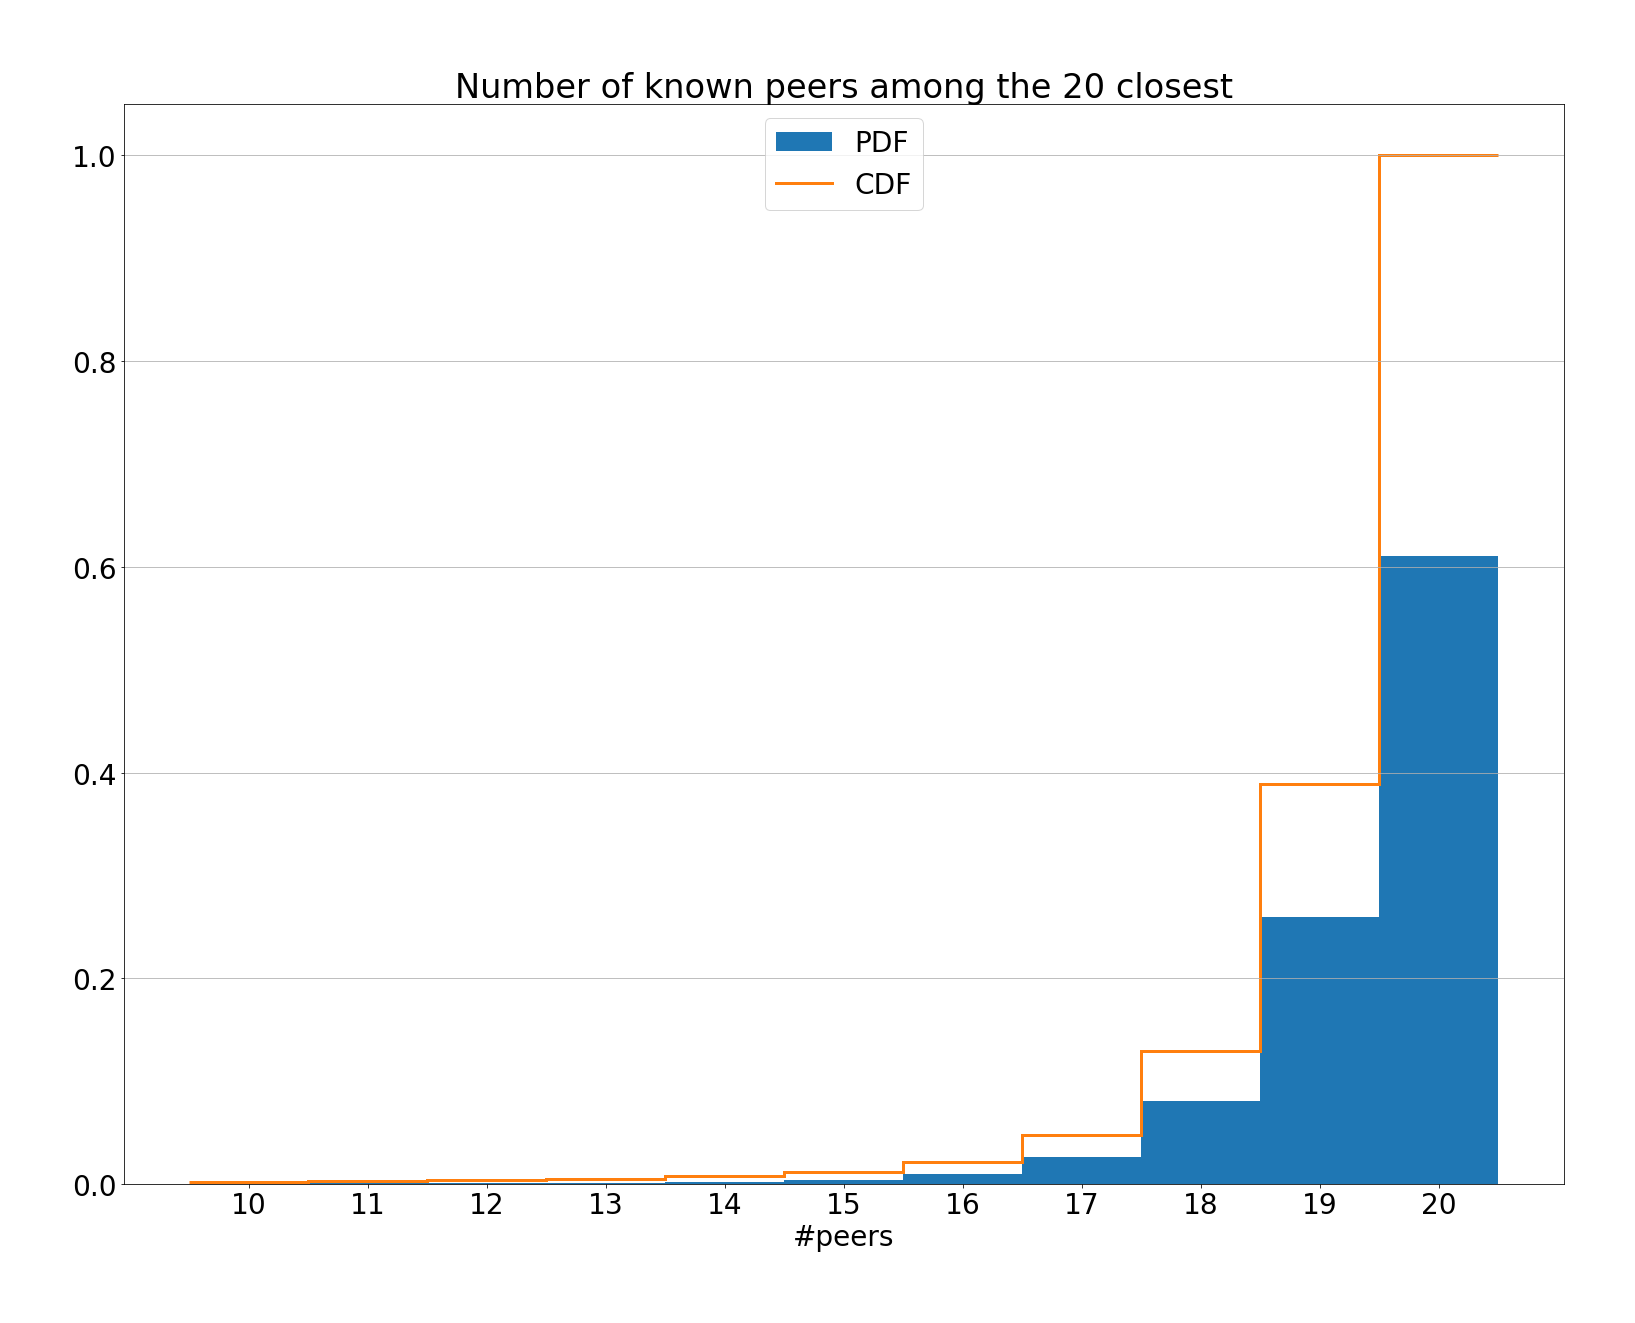
\includegraphics[width=\textwidth]{plots/known-peers-among-20-closest.png}
    \end{center}
\end{column}
\end{columns}
\end{frame}

\begin{frame}
\frametitle{Diversity in the k-buckets}

\begin{itemize}
	\itemc Live peers never get replaced in the \texttt{k-buckets} by design
	\itemc Eventually, buckets with many candidates (e.g buckets \texttt{0-1}) will be filled almost exclusively with a small number of very stable peers
	\itemc Routing for content \textit{far away} (in XOR distance) may become centralized on a small set of peers
	\itemc Bad for decentralization :(
	\itemc Bad for load balancing :(
\end{itemize}
\end{frame}

\iffalse

\begin{frame}
\frametitle{Replacement in action: views of \texttt{buckets 0}}
\textbf{{\color{verystable}Very stable nodes} - {\color{stableenough}Stable enough nodes} - {\color{unstable}Unstable nodes}}

\begin{tikzpicture}[
  thick,
  minimum size=5mm,
  node distance=0.7cm and 3cm,
  >=stealth,
  bend angle=45,
  scale=0.9,
  every node/.style={scale=0.9},
  auto
]

\node (node0)  [rounded corners, align=center, draw=text-color,
             label=above:{\color{verystable}\textbf{node0}}] {
             \begin{minipage}[t][2.2cm]{1.2cm}
             \textbf{{\color{stableenough}node1}\\
              	{\color{unstable}node2}\\
              	{\color{unstable}node3}\\
              	{\color{verystable}node4}\\
              	{\color{stableenough}node5}\\
             }
			\end{minipage}

             };
\node (node1)  [rounded corners, align=center, draw=text-color, below=of node0,
             label=above:{\color{stableenough}\textbf{node1}}] {
             \begin{minipage}[t][2.2cm]{1.2cm}
             \textbf{{\color{verystable}node0}\\
              	{\color{unstable}node2}\\
              	{\color{unstable}node6}\\
              	{\color{unstable}node7}\\
              	{\color{stableenough}node8}\\
             }
			\end{minipage}

             };
            
\node (node2)  [rounded corners, align=center, draw=text-color, right=of node0,
             label=above:{\color{unstable}\textbf{node2}}] {
             \begin{minipage}[t][2.2cm]{1.2cm}
             \textbf{{\color{stableenough}node1}\\
              	{\color{unstable}node3}\\
              	{\color{verystable}node4}\\
              	{\color{stableenough}node5}\\
              	{\color{unstable}node7}\\
             }
			\end{minipage}

             };

\node (node3)  [rounded corners, align=center, draw=text-color, right=of node1,
             label=above:{\color{unstable}\textbf{node3}}] {
             \begin{minipage}[t][2.2cm]{1.2cm}
             \textbf{{\color{verystable}node0}\\
				{\color{stableenough}node1}\\
              	{\color{unstable}node2}\\
              	{\color{verystable}node4}\\
              	{\color{stableenough}node8}\\
             }
			\end{minipage}

             };
\node (node4)  [rounded corners, align=center, draw=text-color, right=of node2,
             label=above:{\color{verystable}\textbf{node4}}] {
             \begin{minipage}[t][2.2cm]{1.2cm}
             \textbf{{\color{stableenough}node1}\\
                {\color{unstable}node3}\\
              	{\color{unstable}node7}\\
                {\color{stableenough}node8}\\
             	{\color{verystable}node10}\\
             }
			\end{minipage}

             };

\node (node5)  [rounded corners, align=center, draw=text-color, right=of node3,
             label=above:{\color{stableenough}\textbf{node5}}] {
             \begin{minipage}[t][2.2cm]{1.2cm}
             \textbf{{\color{stableenough}node1}\\
              	{\color{unstable}node2}\\
              	{\color{unstable}node3}\\
              	{\color{verystable}node4}\\
              	{\color{stableenough}node5}\\
             }
			\end{minipage}

             };

\end{tikzpicture}
\end{frame}

\begin{frame}
\frametitle{Replacement in action: views of \texttt{buckets 0}}
\textbf{{\color{verystable}Very stable nodes} - {\color{stableenough}Stable enough nodes} - {\color{unstable}Unstable nodes}}

\begin{tikzpicture}[
  thick,
  minimum size=5mm,
  node distance=0.7cm and 3cm,
  >=stealth,
  bend angle=45,
  scale=0.9,
  every node/.style={scale=0.9},
  auto
]

\node (node0)  [rounded corners, align=center, draw=text-color,
             label=above:{\color{verystable}\textbf{node0}}] {
             \begin{minipage}[t][2.2cm]{1.2cm}
             \textbf{{\color{stableenough}node1}\\
              	\sout{node2}\\
              	\sout{node3}\\
              	{\color{verystable}node4}\\
              	{\color{stableenough}node5}\\
             }
			\end{minipage}

             };
\node (node1)  [rounded corners, align=center, draw=text-color, below=of node0,
             label=above:{\color{stableenough}\textbf{node1}}] {
             \begin{minipage}[t][2.2cm]{1.2cm}
             \textbf{{\color{verystable}node0}\\
              	\sout{node2}\\
              	\sout{node6}\\
              	\sout{node7}\\
              	{\color{stableenough}node8}\\
             }
			\end{minipage}

             };
            
\node (node2)  [rounded corners, align=center, draw=text-color, right=of node0,
             label=above:\sout{node2}] {
             \begin{minipage}[t][2.2cm]{1.2cm}
             \sout{node1}\\
              	\sout{node3}\\
              	\sout{node4}\\
              	\sout{node5}\\
              	\sout{node7}\\
			\end{minipage}
             };
             
\node (node3)  [rounded corners, align=center, draw=text-color, right=of node1,
             label=above:\sout{node3}] {
             \begin{minipage}[t][2.2cm]{1.2cm}
             \sout{node0}\\
              	\sout{node1}\\
              	\sout{node2}\\
              	\sout{node4}\\
              	\sout{node8}\\
			\end{minipage}
             };

\node (node4)  [rounded corners, align=center, draw=text-color, right=of node2,
             label=above:{\color{verystable}\textbf{node4}}] {
             \begin{minipage}[t][2.2cm]{1.2cm}
             \textbf{{\color{stableenough}node1}\\
                \sout{node3}\\
              	\sout{node7}\\
                {\color{stableenough}node8}\\
             	{\color{verystable}node10}\\
             }
			\end{minipage}

             };

\node (node5)  [rounded corners, align=center, draw=text-color, right=of node3,
             label=above:{\color{stableenough}\textbf{node5}}] {
             \begin{minipage}[t][2.2cm]{1.2cm}
             \textbf{{\color{stableenough}node1}\\
              	\sout{node2}\\
              	\sout{node3}\\
              	{\color{verystable}node4}\\
              	{\color{stableenough}node5}\\
             }
			\end{minipage}

             };

\end{tikzpicture}
\end{frame}

\begin{frame}
\frametitle{Replacement in action: views of \texttt{buckets 0}}
\textbf{{\color{verystable}Very stable nodes} - {\color{stableenough}Stable enough nodes} - {\color{unstable}Unstable nodes}}
\begin{tikzpicture}[
  thick,
  minimum size=5mm,
  node distance=0.7cm and 3cm,
  >=stealth,
  bend angle=45,
  scale=0.9,
  every node/.style={scale=0.9},
  auto
]

\node (node0)  [rounded corners, align=center, draw=text-color,
             label=above:{\color{verystable}\textbf{node0}}] {
             \begin{minipage}[t][2.2cm]{1.2cm}
             \textbf{{\color{stableenough}node1}\\
              	{\color{unstable}node20}\\
              	{\color{verystable}node11}\\
              	{\color{verystable}node4}\\
              	{\color{stableenough}node5}\\
             }
			\end{minipage}

             };
\node (node1)  [rounded corners, align=center, draw=text-color, below=of node0,
             label=above:{\color{stableenough}\textbf{node1}}] {
             \begin{minipage}[t][2.2cm]{1.2cm}
             \textbf{{\color{verystable}node0}\\
              	{\color{verystable}node12}\\
              	{\color{unstable}node21}\\
              	{\color{stableenough}node13}\\
              	{\color{stableenough}node8}\\
             }
			\end{minipage}

             };
            
\node (node2)  [rounded corners, align=center, draw=text-color, right=of node0,
             label=above:{\color{unstable}\textbf{node20}}] {
             \begin{minipage}[t][2.2cm]{1.2cm}
             \textbf{{\color{verystable}node0}\\
				{\color{stableenough}node1}\\
              	{\color{verystable}node4}\\
              	{\color{stableenough}node5}\\
              	{\color{unstable}node21}\\
             }
			\end{minipage}

             };

\node (node3)  [rounded corners, align=center, draw=text-color, right=of node1,
             label=above:{\color{unstable}\textbf{node21}}] {
             \begin{minipage}[t][2.2cm]{1.2cm}
             \textbf{{\color{verystable}node0}\\
              	{\color{verystable}node4}\\
              	{\color{stableenough}node5}\\
              	{\color{stableenough}node8}\\
              	{\color{verystable}node12}\\
             }
			\end{minipage}

             };
\node (node4)  [rounded corners, align=center, draw=text-color, right=of node2,
             label=above:{\color{verystable}\textbf{node4}}] {
             \begin{minipage}[t][2.2cm]{1.2cm}
             \textbf{{\color{stableenough}node1}\\
                {\color{stableenough}node8}\\
             	{\color{verystable}node10}\\
              	{\color{verystable}node12}\\
              	{\color{stableenough}node15}\\
             }
			\end{minipage}

             };

\node (node5)  [rounded corners, align=center, draw=text-color, right=of node3,
             label=above:{\color{stableenough}\textbf{node5}}] {
             \begin{minipage}[t][2.2cm]{1.2cm}
             \textbf{{\color{stableenough}node1}\\
              	{\color{verystable}node4}\\
              	{\color{stableenough}node5}\\
              	{\color{stableenough}node8}\\
              	{\color{unstable}node21}\\
             }
			\end{minipage}

             };

\end{tikzpicture}
\end{frame}


\begin{frame}
\frametitle{Replacement in action: views of \texttt{buckets 0}}
\textbf{{\color{verystable}Very stable nodes} - {\color{stableenough}Stable enough nodes} - {\color{unstable}Unstable nodes}}
\begin{tikzpicture}[
  thick,
  minimum size=5mm,
  node distance=0.7cm and 3cm,
  >=stealth,
  bend angle=45,
  scale=0.9,
  every node/.style={scale=0.9},
  auto
]

\node (node0)  [rounded corners, align=center, draw=text-color,
             label=above:{\color{verystable}\textbf{node0}}] {
             \begin{minipage}[t][2.2cm]{1.2cm}
             \textbf{\sout{node1}\\
              	\sout{node20}\\
              	{\color{verystable}node11}\\
              	{\color{verystable}node4}\\
              	\sout{node5}\\
             }
			\end{minipage}

             };
\node (node1)  [rounded corners, align=center, draw=text-color, below=of node0,
             label=above:\sout{node1}] {
             \begin{minipage}[t][2.2cm]{1.2cm}
             \sout{node0}\\
              \sout{node12}\\
              \sout{node21}\\
              \sout{node13}\\
              \sout{node8}\\
          
			\end{minipage}

             };
            
\node (node2)  [rounded corners, align=center, draw=text-color, right=of node0,
             label=above:\sout{node20}] {
             \begin{minipage}[t][2.2cm]{1.2cm}
             \sout{node0}\\
			 \sout{node1}\\
             \sout{node4}\\
              \sout{node5}\\
              \sout{node21}\\
             
			\end{minipage}

             };

\node (node3)  [rounded corners, align=center, draw=text-color, right=of node1,
             label=above:\sout{node21}] {
             \begin{minipage}[t][2.2cm]{1.2cm}
             \sout{node0}\\
             \sout{node4}\\
             \sout{node5}\\
             \sout{node8}\\
             \sout{node12}\\
			\end{minipage}

             };
\node (node4)  [rounded corners, align=center, draw=text-color, right=of node2,
             label=above:{\color{verystable}\textbf{node4}}] {
             \begin{minipage}[t][2.2cm]{1.2cm}
             \textbf{\sout{node1}\\
                \sout{node8}\\
             	{\color{verystable}node10}\\
              	{\color{verystable}node12}\\
              	\sout{node15}\\
             }
			\end{minipage}

             };

\node (node5)  [rounded corners, align=center, draw=text-color, right=of node3,
             label=above:\sout{node5}] {
             \begin{minipage}[t][2.2cm]{1.2cm}
             \sout{node1}\\
             \sout{node4}\\
             \sout{node5}\\
             \sout{node8}\\
             \sout{node21}\\
			\end{minipage}

             };

\end{tikzpicture}
\end{frame}

\begin{frame}
\frametitle{Replacement in action: views of \texttt{buckets 0}}
\textbf{{\color{verystable}Very stable nodes} - {\color{stableenough}Stable enough nodes} - {\color{unstable}Unstable nodes}}
\begin{tikzpicture}[
  thick,
  minimum size=5mm,
  node distance=0.7cm and 3cm,
  >=stealth,
  bend angle=45,
  scale=0.9,
  every node/.style={scale=0.9},
  auto
]

\node (node0)  [rounded corners, align=center, draw=text-color,
             label=above:{\color{verystable}\textbf{node0}}] {
             \begin{minipage}[t][2.2cm]{1.2cm}
             \textbf{
              	{\color{verystable}node4}\\
              	{\color{verystable}node11}\\
              	{\color{verystable}node23}\\
              	{\color{verystable}node32}\\
              	{\color{verystable}node35}\\
             }
			\end{minipage}

             };
\node (node1)  [rounded corners, align=center, draw=text-color, below=of node0,
             label=above:\sout{node1}] {
             \begin{minipage}[t][2.2cm]{1.2cm}
             \sout{node0}\\
              \sout{node12}\\
              \sout{node21}\\
              \sout{node13}\\
              \sout{node8}\\
          
			\end{minipage}

             };
            
\node (node2)  [rounded corners, align=center, draw=text-color, right=of node0,
             label=above:\sout{node20}] {
             \begin{minipage}[t][2.2cm]{1.2cm}
             \sout{node0}\\
			 \sout{node1}\\
             \sout{node4}\\
              \sout{node5}\\
              \sout{node21}\\
             
			\end{minipage}

             };

\node (node3)  [rounded corners, align=center, draw=text-color, right=of node1,
             label=above:\sout{node21}] {
             \begin{minipage}[t][2.2cm]{1.2cm}
             \sout{node0}\\
             \sout{node4}\\
             \sout{node5}\\
             \sout{node8}\\
             \sout{node12}\\
			\end{minipage}

             };
\node (node4)  [rounded corners, align=center, draw=text-color, right=of node2,
             label=above:{\color{verystable}\textbf{node4}}] {
             \begin{minipage}[t][2.2cm]{1.2cm}
             \textbf{{\color{verystable}node0}\\
             	{\color{verystable}node10}\\
              	{\color{verystable}node12}\\
             	{\color{verystable}node23}\\
              	{\color{verystable}node32}\\
             }
			\end{minipage}

             };

\node (node5)  [rounded corners, align=center, draw=text-color, right=of node3,
             label=above:\sout{node5}] {
             \begin{minipage}[t][2.2cm]{1.2cm}
             \sout{node1}\\
             \sout{node4}\\
             \sout{node5}\\
             \sout{node8}\\
             \sout{node21}\\
			\end{minipage}

             };

\end{tikzpicture}
\end{frame}

\begin{frame}
\frametitle{Replacement in action: views of \texttt{buckets 0}}
\textbf{{\color{verystable}Very stable nodes} - {\color{stableenough}Stable enough nodes} - {\color{unstable}Unstable nodes}}
\begin{tikzpicture}[
  thick,
  minimum size=5mm,
  node distance=0.7cm and 3cm,
  >=stealth,
  bend angle=45,
  scale=0.9,
  every node/.style={scale=0.9},
  auto
]

\node (node0)  [rounded corners, align=center, draw=text-color,
             label=above:{\color{verystable}\textbf{node0}}] {
             \begin{minipage}[t][2.2cm]{1.2cm}
             \textbf{
              	{\color{verystable}node4}\\
              	{\color{verystable}node11}\\
              	{\color{verystable}node23}\\
              	{\color{verystable}node32}\\
              	{\color{verystable}node35}\\
             }
			\end{minipage}

             };
\node (node1)  [rounded corners, align=center, draw=text-color, below=of node0,
             label=above:{\color{stableenough}\textbf{node36}}] {
             \begin{minipage}[t][2.2cm]{1.2cm}
             \textbf{
              	{\color{verystable}node4}\\
              	{\color{verystable}node11}\\
              	{\color{verystable}node12}\\
             	{\color{verystable}node23}\\
              	{\color{unstable}node39}\\
             }
			\end{minipage}

             };
            
\node (node2)  [rounded corners, align=center, draw=text-color, right=of node0,
             label=above:{\color{unstable}\textbf{node37}}] {
             \begin{minipage}[t][2.2cm]{1.2cm}
             \textbf{{\color{verystable}node0}\\
              	{\color{verystable}node4}\\
              	{\color{verystable}node12}\\
             	{\color{verystable}node23}\\
              	{\color{verystable}node35}\\
             }
			\end{minipage}

             };

\node (node3)  [rounded corners, align=center, draw=text-color, right=of node1,
             label=above:{\color{unstable}\textbf{node39}}] {
             \begin{minipage}[t][2.2cm]{1.2cm}
             \textbf{{\color{verystable}node0}\\
             	{\color{verystable}node4}\\
              	{\color{verystable}node12}\\
              	{\color{verystable}node32}\\
              	{\color{stableenough}node41}\\
             }
			\end{minipage}

             };
\node (node4)  [rounded corners, align=center, draw=text-color, right=of node2,
             label=above:{\color{verystable}\textbf{node4}}] {
             \begin{minipage}[t][2.2cm]{1.2cm}
             \textbf{{\color{verystable}node0}\\
             	{\color{verystable}node10}\\
              	{\color{verystable}node12}\\
             	{\color{verystable}node23}\\
              	{\color{verystable}node32}\\
             }
			\end{minipage}

             };

\node (node5)  [rounded corners, align=center, draw=text-color, right=of node3,
             label=above:{\color{stableenough}\textbf{node41}}] {
             \begin{minipage}[t][2.2cm]{1.2cm}
             \textbf{{\color{verystable}node0}\\
             	{\color{verystable}node10}\\
              	{\color{verystable}node11}\\
             	{\color{verystable}node23}\\
              	{\color{verystable}node35}\\
             }
			\end{minipage}

             };

\draw[<-, thick] (node0.east) -- (node2.west);
\draw[<-, thick] (node0.east) -- (node3.west);
\draw[<-, thick] (node4.west) -- (node2.east);
\draw[<-, thick] (node4.west) -- (node3.east);

%\draw[->, thick] ([yshift=-0.3cm] peer0.west) -- node[midway, above]{\texttt{Peer1}} ([yshift=-0.3cm] client.east |-peer0.west);


\end{tikzpicture}
\end{frame}

\fi

\begin{frame}
\frametitle{Diversity measurements}
\begin{columns}[onlytextwidth]
\begin{column}{0.38\textwidth}
   \begin{itemize}
   		\itemc Measurements for 10 consecutive weeks starting on \texttt{2022-02-16}
   		\itemc Each week's measurements are based on data from 14 crawls (2x/day)
   		\itemc Diversity in \texttt{k-buckets} is measured as the number of distinct \texttt{peer\_id}s observed in each bucket for all peers
   \end{itemize}
\end{column}
\begin{column}{0.58\textwidth}
    \begin{center}
		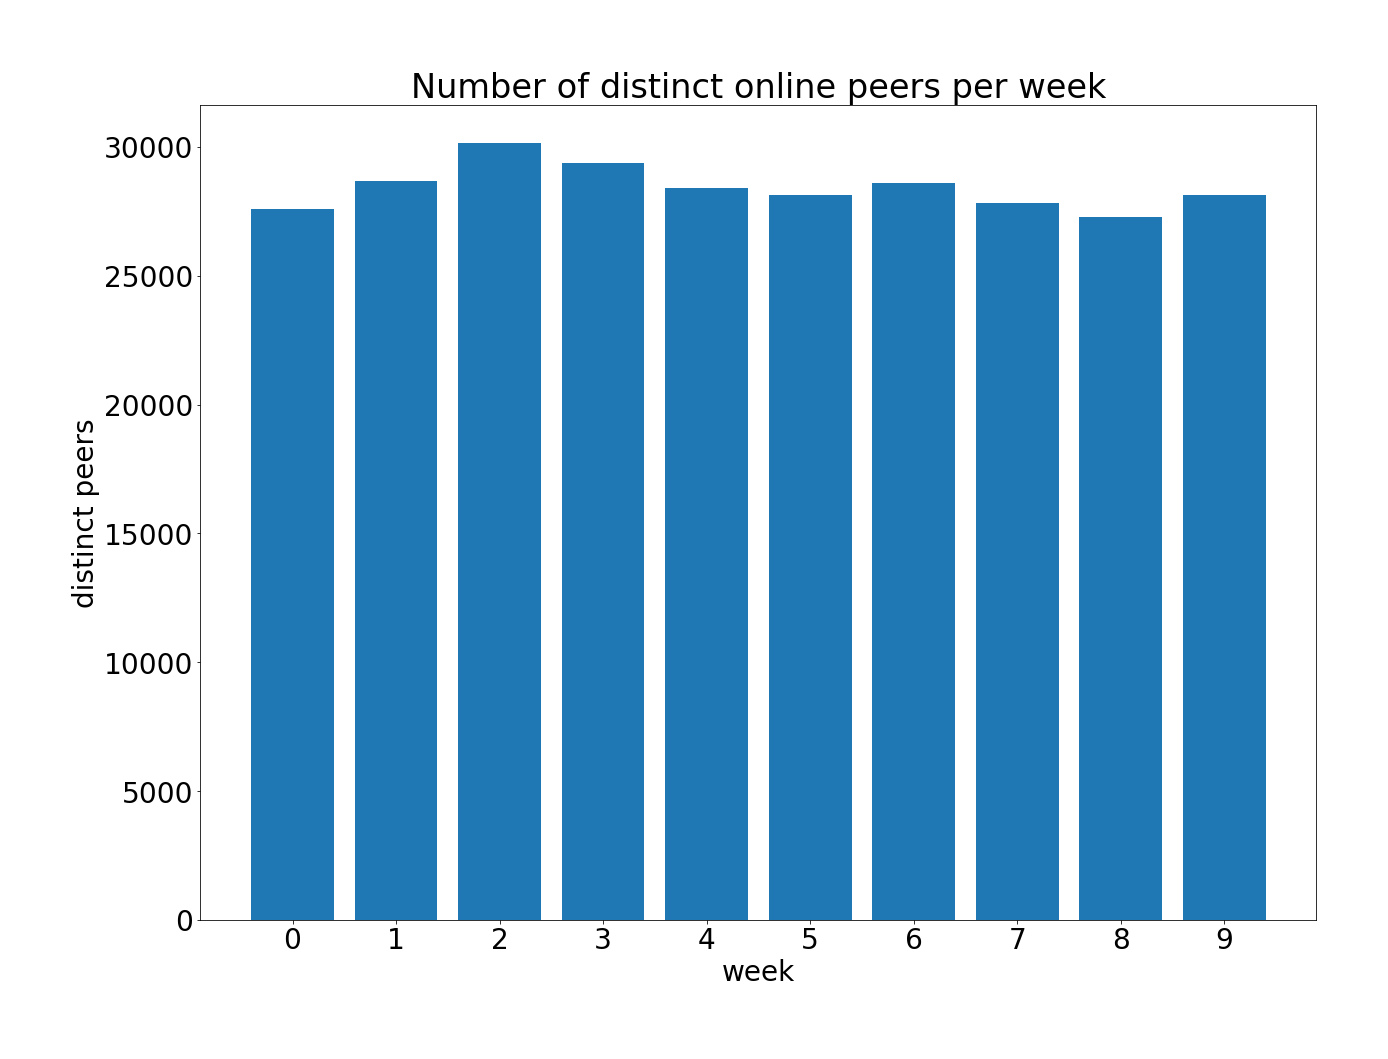
\includegraphics[width=\textwidth]{plots/online-peers-per-week.png}
    \end{center}
\end{column}
\end{columns}
\end{frame}

\begin{frame}
\frametitle{Diversity in each k-buckets}

\begin{columns}[onlytextwidth]
\begin{column}{0.38\textwidth}
   \begin{itemize}
   		\itemc Buckets \texttt{10+}: non-full buckets $\rightarrow$ low diversity
   		\itemc Bucket \texttt{9}: bucket just full \\$\rightarrow$ highest diversity
   		\itemc Buckets \texttt{0-1}: many candidates, only the most stable don't get evicted \\$\rightarrow$ lower diversity
   		\itemc We expect diversity in buckets \texttt{0-1} to decrease over time
   \end{itemize}
\end{column}
\begin{column}{0.58\textwidth}
    \begin{center}
		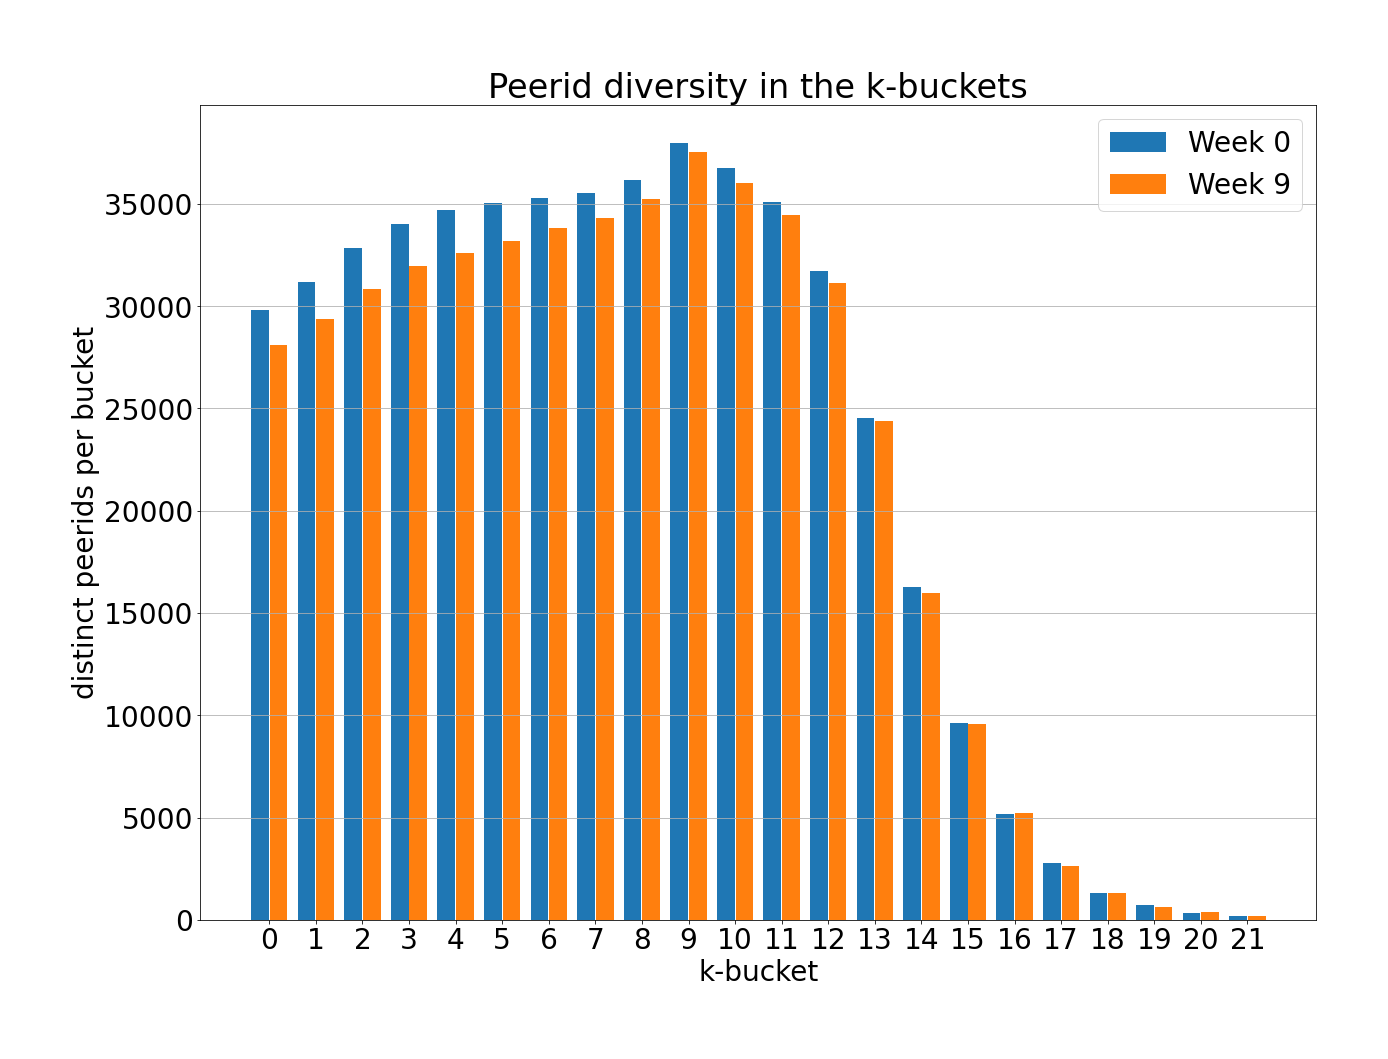
\includegraphics[width=\textwidth]{plots/diversity-in-buckets.png}
    \end{center}
\end{column}
\end{columns}
\end{frame}

\begin{frame}
\frametitle{Diversity evolution over time}

\begin{columns}[onlytextwidth]
\begin{column}{0.38\textwidth}
   Moving average difference between week 1 and week 8:
   \begin{itemize}
   		\item[] Bucket 0: \hspace{1em}\textbf{-6.9\%}
   		\item[] Bucket 1: \hspace{1em}\textbf{-7.3\%}
   		\item[] Bucket 9: \hspace{1em}-2.6\%
   \end{itemize}
\end{column}
\begin{column}{0.58\textwidth}
    \begin{center}
		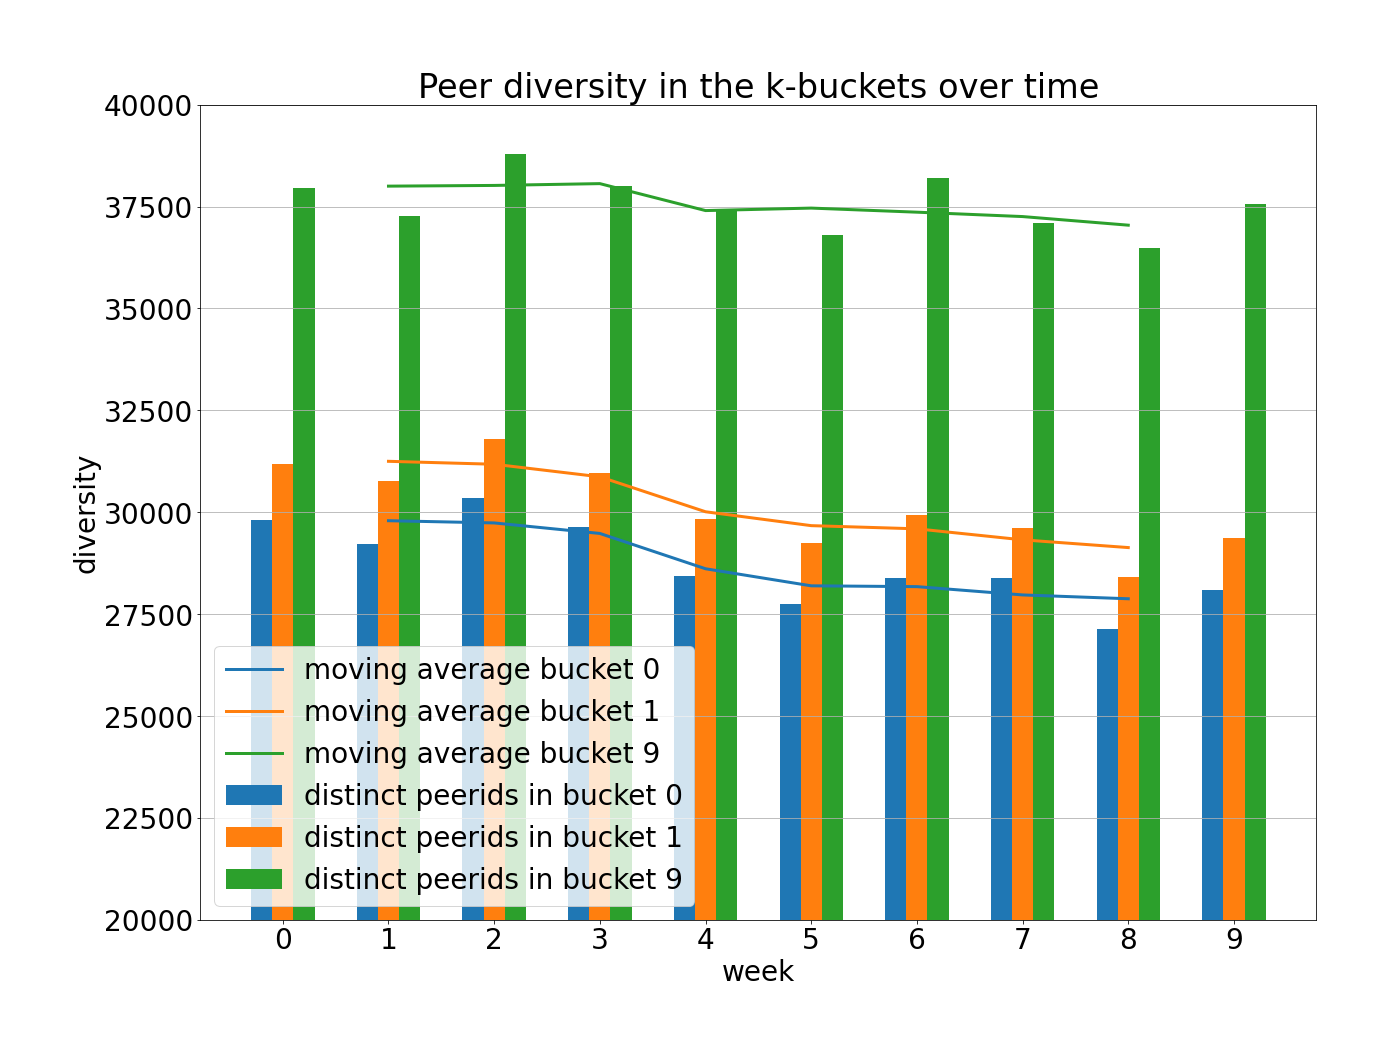
\includegraphics[width=\textwidth]{plots/diversity-b0-b1-b9.png}
    \end{center}
\end{column}
\end{columns}
\end{frame}

\begin{frame}
\frametitle{Persisting Routing Table States}

\begin{itemize}
	\itemc Routing table currently flushed upon node shutdown
	\itemc Routing table has to be repopulated on restart, using bootstrap peers
\end{itemize}
\vspace{2em}
Persisting the state of the routing table would allow:
\smallskip
\begin{itemize}
	\itemc Faster convergence
	\itemc Less dependence on bootstrap nodes
\end{itemize}
\end{frame}

\begin{frame}
\frametitle{DHT connection graph}
\begin{minipage}[b]{.49\linewidth}
\begin{center}
        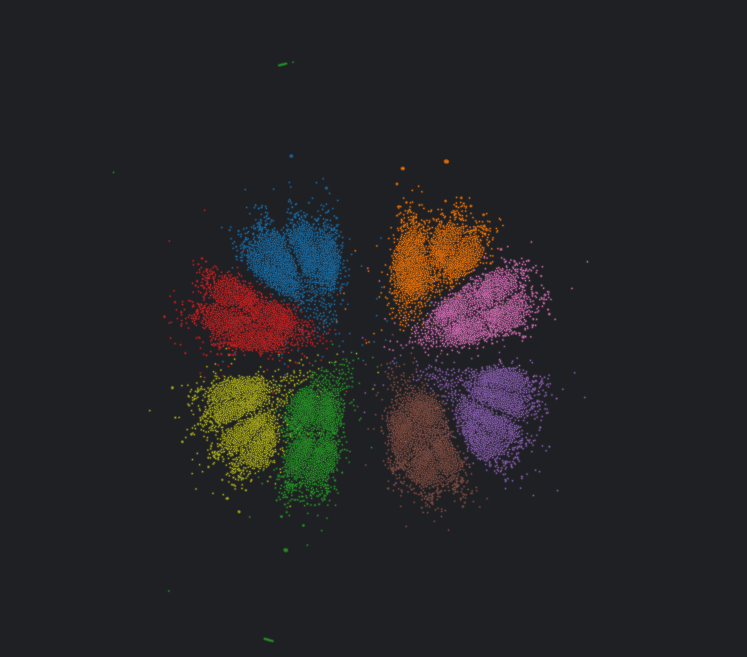
\includegraphics[width=\linewidth,keepaspectratio]{resources/dht-graph.png}
\end{center}
\end{minipage}
\begin{minipage}[b]{.49\linewidth}
\begin{center}
        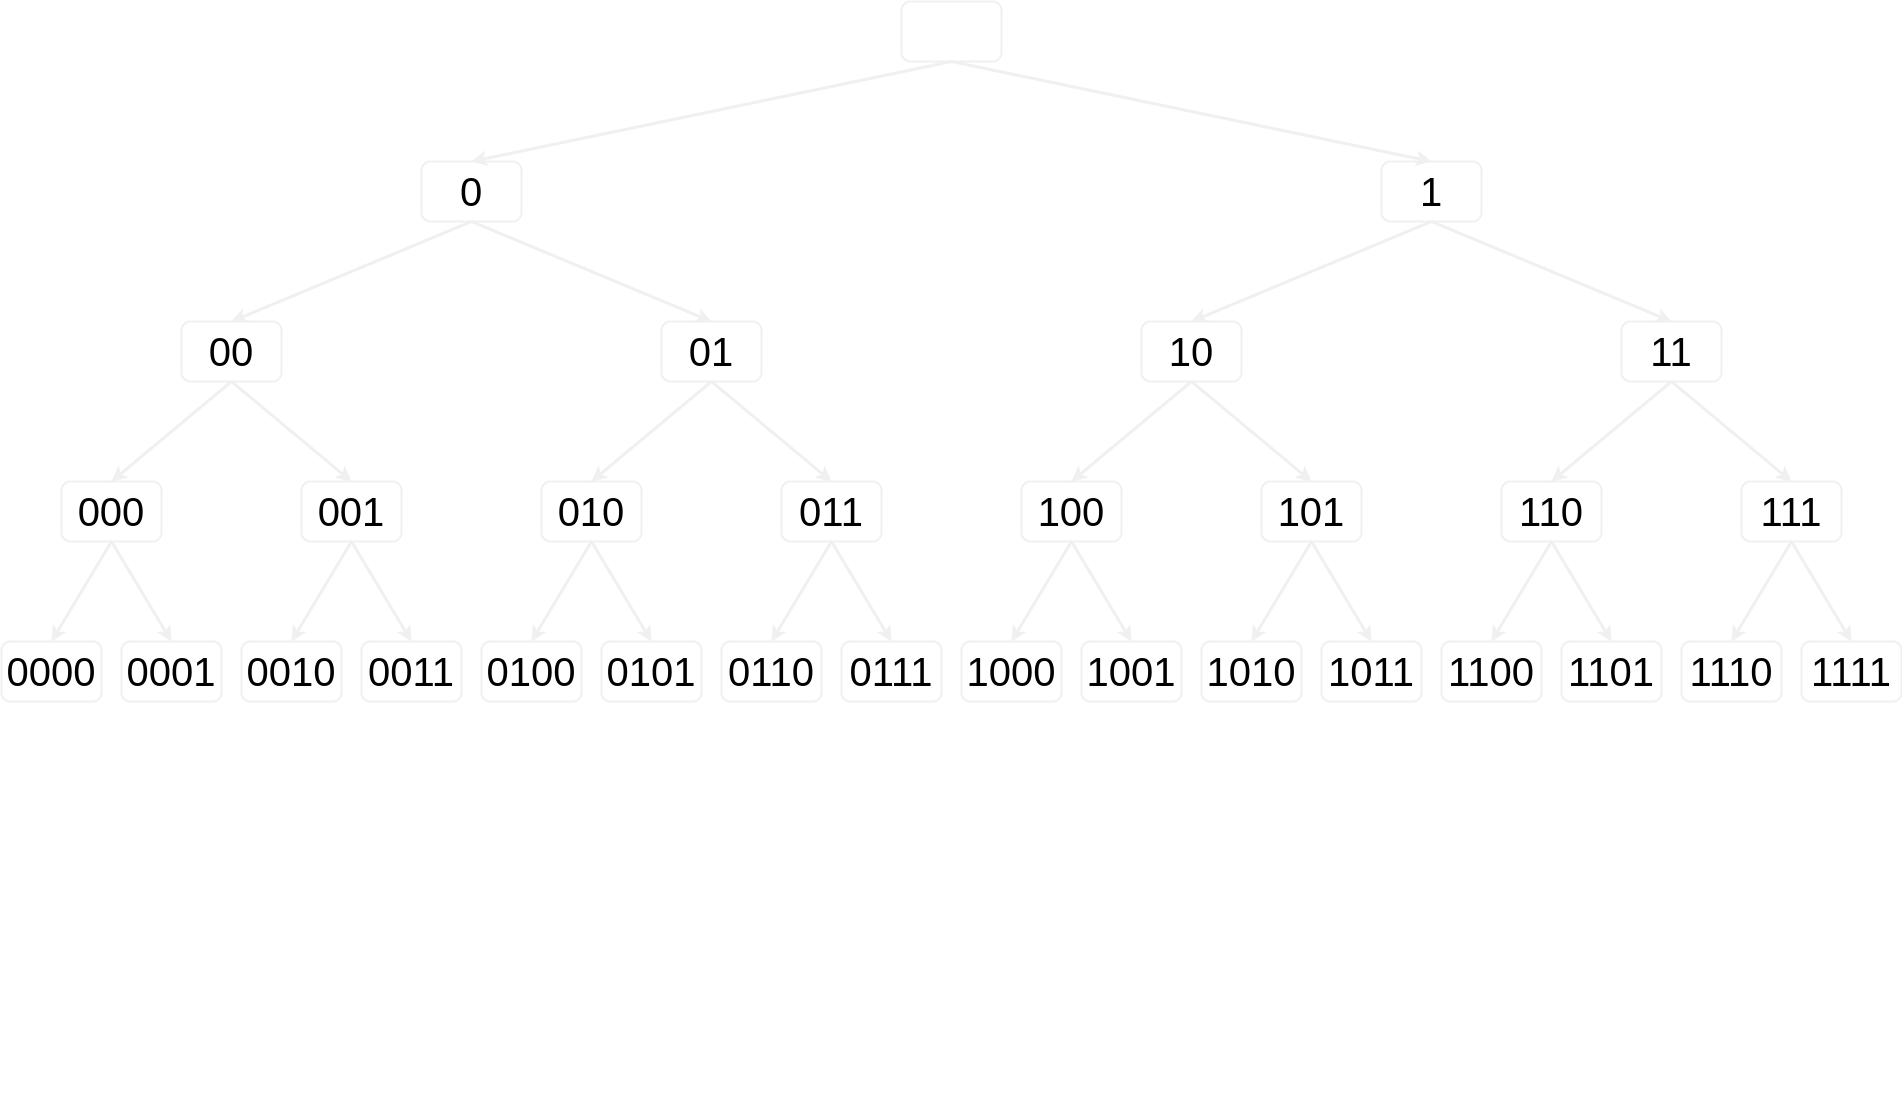
\includegraphics[width=\linewidth,keepaspectratio]{resources/dht-vanilla.png}
\end{center}
\end{minipage}

\end{frame}


\begin{frame}
\frametitle{Conclusion}
\begin{itemize}
	\itemc Very low rate of stale entries in the routing table, given high churn
	\itemc Peers distributions in the \texttt{k-buckets} as expected
	\itemc The \texttt{k-buckets} are only missing a small number of peers
	\itemc \texttt{95.2\%} of the nodes have at least 18 of their 20 closest peers in their Routing Table
	\itemc We observed diversity decreasing over time in low ID buckets, which might become a concern for decentralization
	\bigskip
	%\itemc All results of \hyperlink{https://github.com/protocol/network-measurements/blob/rfm19/results/rfm19-dht-routing-table-health.md}{\texttt{RFM19}} of are available on the \hyperlink{https://github.com/protocol/network-measurements}{\texttt{protocol/network-measurements}} Github repo
\end{itemize}
\end{frame}

\begin{frame}
\frametitle{References}
\begin{center}
Complete report available
\medskip

\qrcode[height=4cm]{https://github.com/protocol/network-measurements/blob/rfm19/results/rfm19-dht-routing-table-health.md}

\medskip
https://github.com/protocol/network-measurements
\end{center}
\end{frame}

\begin{frame}
\frametitle{Digression: Bucket quotas}
\begin{center}
	{\large\greencube \hspace{1em} \textit{Make the bucket replacement policy smarter} \hspace{1em}\greencube}
\end{center}
\bigskip
\begin{itemize}
	\itemc Reduce number of hops
	\itemc Reduce hop latency
	\itemc More load balancing through diversity
	\itemc Make the DHT agile and upgradable
	\itemc Keep DHT stability
\end{itemize}
\end{frame}

\begin{frame}
\frametitle{Current quotas}
\begin{itemize}
	\itemc No more than 3 IP addresses from the same Autonomous System (AS) in the routing table
	\itemc No more than 2 IP addresses from the same AS in the same bucket
\end{itemize}
\end{frame}

\begin{frame}
\frametitle{Quotas example}
Out of the 20 peers per bucket, if possible we want:
\begin{itemize}
	\itemc The 5 nodes with the longest uptime
	\itemc 5 nodes whose RTT is below the 30th percentile of this bucket candidates' RTT
	\itemc 1 node in each of the 4 sub-buckets (4 in total)
	\itemc 4 peers whose DHT version is higher or equal to its own version
	\itemc 2 random peers
\end{itemize}
Nodes from the low RTT, DHT version and random peers get probabilistically pruned and replaced, e.g every 6 hours one node is pruned.\\
\smallskip
Note: peers can belong to multiple categories at once.
\end{frame}

\begin{frame}
\frametitle{Side effects}
\begin{itemize}
	\itemc Close buckets (high ID) will not change
	\itemc Far buckets (low ID) are expected to change
	\itemc Stable up-to-date central nodes will be easy to find
	\itemc Reaching unstable outdated nodes with high latency may require one extra hop
	\itemc Lookup latency (finding 1 of the 20 closest nodes to a key) is expected to significantly decrease
	\itemc Provide latency (finding the 20 closest nodes to a key) is expected to slightly decrease
\end{itemize}
\end{frame}

\end{document}